% Document
\documentclass[12pt, a4paper]{article}
\usepackage[T1]{fontenc}
\usepackage[utf8]{inputenc}
\usepackage{authblk}
\usepackage{lipsum}

% Figure and table formating
\usepackage{epsfig}
\usepackage{tabu}
\usepackage{rotating}
\usepackage{pbox}
\usepackage{framed, multicol}
\usepackage[framemethod=TikZ]{mdframed}
\usepackage{float}
\usepackage[left=1.25 in, right=1.25 in, top=1.25 in, bottom=1.25 in]{geometry}

% Fonts - Mathtime
%\usepackage{txfonts}
\usepackage{amsmath} % Add amssymb if not using Mathtime

% Text
\setlength{\parindent}{0.5in}
\frenchspacing  \tolerance = 800  \hyphenpenalty = 800

\usepackage{lineno} % Line numbers
\def\linenumberfont{\normalfont\footnotesize\ttfamily}
\setlength\linenumbersep{0.2 in}

\usepackage{setspace}

% Format section and subsection headers
\makeatletter
\renewcommand{\section}{\@startsection
{section}%                   % the name
{1}%                         % the level
{0mm}%                       % the indent
{-\baselineskip}%            % the before skip
{0.5\baselineskip}%          % the after skip
{\normalfont\bf\large}} % the style

\renewcommand{\subsection}{\@startsection
{subsection}%                   % the name
{2}%                         % the level
{0mm}%                       % the indent
{-\baselineskip}%            % the before skip
{0.5\baselineskip}%          % the after skip
{\normalfont\bf}} % the style
\makeatother

% Other
\usepackage{graphicx}
\usepackage[singlelinecheck=false,font=small,labelfont=bf]{caption}

% Bibliography
\usepackage[numbers, compress]{natbib} % Bibliography - APA
\bibpunct{(}{)}{;}{a}{}{,}

% Format the Bibliography appropriately
% increase \bibhang to take care of the numbers
\setlength{\bibhang}{0pc}
\makeatletter
% patch \@lbibitem to print the current number before the authors
\patchcmd{\@lbibitem}
  {]}
  {] \theNAT@ctr. \newline }
  {}{}
\makeatother


%%%%%% FRONT MATTER %%%%%%%%%

\begin{document}

\linenumbers

\doublespacing

\noindent
\Large{\textbf{Supporting Information}}

\normalsize

\section*{Appendix 1: Implementation of the Crofton Method}

The algorithm for fitting the Crofton Method \citep{Crofton1971a} proceeds as follows. First, obtain a dataset
with $n$ hosts where each host has some parasite intensity 0 to $p_{max}$. Starting
with the full dataset, guess a vector of pre-mortality parameters $(N_p, \mu_p, k_p)$ and given
these parameters calculate the predicted number of hosts with $0, 1, 2, \dots
p_{max}$.  Compare the expected number of hosts with $0, 1, 2, \dots  p_{max}$ parasites
to the observed number hosts with $0, 1, 2, \dots p_{max}$ parasites and calculate
the $\chi^2$-squared statistic associated with your observed and predicted vectors. In reality, one often has to bin the parasite intensity data because all
parasite intensities are not represented in the dataset. Continue to guess $(N_p,
mu_p, k_p)$ vectors until a set of parameters is found that minimizes the $\chi^2$-
squared statistic.

Second, choose a truncation value ($t_1$) such that $t_1 <
p_{max}$. Truncate the data such that $\text{data}_\text{truncated} <= t$ and repeat the above
iterative procedure to calculate another set of parameters $(N_{p2}, \mu_{p2}, k_{p2})$
that minimizes the $\chi^2$-squared statistic on the truncated data. Choose a new
truncated value $t_2 < t_1$ and repeat the first two steps. Continue to truncated
the dataset until it only contains hosts with 0, 1, and 2 parasites (or 3 bins).
As the method attempts to estimate three parameters, at least 3 classes are
needed if all 3 parameters are to be identifiable \citep{Royce1990}.

We provide an implementation and unit tests of the Crofton Method Supplementary Information 4.  Figure \ref{fig:crof_test} visually shows that our implementation of the Crofton Method agrees with results previously published by \cite{Crofton1971a}.

\section*{Appendix 2: Implementation of the Adjei Method}

The Adjei Method for estimating PIHM has two steps \citep{Adjei1986}.  The first
step is to estimate the parameters of the pre-mortality host-parasite
distribution using the Crofton Method.  The three parameters estimated are the
total number of hosts before mortality $N_p$,  the mean number of parasites per
host before mortality $\mu_p$, and the aggregation of parasites before
mortality given by the parameter $k_p$ from a negative binomial distribution.
When $k_p$ is small, parasites are highly aggregated among hosts and when
$k_p$ is large parasites are more evenly spread out \citep{Wilson2002}.  The implementation of the Crofton Method has been discussed at length elsewhere \citep[e.g.][ and above]{Royce1990,Lester1984} and we provide a tested implementation of the method in SI 4.

The second step of the Adjei Method is to estimate the shape of the host survival function. \cite{Adjei1986} assume that the host survival function follows the logistic form

\begin{equation}
    h(x | a, b) = h_x = \dfrac{e^{a - b \log(x)}}{1 + e^{a - b \log(x)}}
    \label{eq:logistic}
\end{equation}
where $x$ is the parasite intensity in a given host and $a$ and $b$ are the two
parameters of the logistic function. Generally, a larger $a$ allows for hosts to
tolerate larger parasite intensities before experiencing parasite-induced mortality
and a larger $b$ leads to a more rapid decline in the probability of host
survival as parasite intensity increases.  The value $\exp(a / b)$ is referred
to as the $LD_{50}$, which gives the parasite intensity at which 50\% of hosts
experience mortality.

To estimate this function, the Adjei Method first
calculates the expected number of hosts with a given parasite load $x$ by using
the equation $g(x ; \mu_p, k_p) * N_p$, where $g(x ; \cdot)$ is the negative binomial pre-mortality distribution.  Second, the observed and predicted number of hosts
with $x$ parasites are paired as a single data point and the method then assumes that
this data point follows a binomial distribution with the total number of
``trials'' equal to the predicted number of hosts and the total number of
``successes'' equal to the observed number of hosts. In some cases, the
observed number of hosts is greater than the expected number of hosts and the
Adjei Method alters the data so that the observed is equal to the predicted
\citep{Adjei1986}.  After this questionable manipulation, the (observed, predicted) pairs are fit to a standard Generalized Linear Model \citep{McCullagh1989} with a binomial response variable and a logistic link function given by equation \ref{eq:logistic}.  This model provides estimates for parameters $a$, $b$ and $LD_{50}$.

While not included in the original implementation of the Adjei Method, a
$\chi^2$ test with a degrees of freedom of 1 can be used to assess whether a GLM model that includes parasite
intensity as a predictor of host survival probability is a ``better'' model than a
GLM without this predictor.  This allows the Adjei Method to determine whether
PIHM is a significant factor in a host-parasite system.

The Adjei Method's most glaring deficiency is the need to alter the observed
data in order to fit the model into the binomial GLM framework.  A second more
subtle problem with the Adjei Method is the potential need to bin data in order
to predict greater than one host in a given parasite intensity class.  For
example, if the total number of hosts pre-mortality was 50, the mean number of
parasites per host pre-mortality was 100 and the aggregation parameter was 1, applying the equation $g(x ; \mu_p=100, k_p=1) * 50$ would result in
less than 1 individual in all parasite intensities $x$. In other words, the
Adjei Method cannot be applied to samples with either very high mean parasite
loads, small sample sizes, or both without some sort of binning of the data.
While this is not a flaw \emph{per se}, it does add a certain level of
subjectivity (i.e. which bins should you use?) to a method that already has
serious potential issues.  In this analysis, we always assume the Adjei Method is not binning the data, though we provide code for applying the binning method in SI 4.

% \section*{Appendix 3: Implementation of the Likelihood Method}

% As described in the main text, the probability mass function for the likelihood method is given by


% \begin{equation}
%     P(x | \text{survival}) = \dfrac{P(\text{survival} | x) * P(x)}{P(\text{survival})}
%     \label{eq:concept}
% \end{equation}

% One can see that $P(\text{survival} | x)$ is the survival function $h(x; a, b)$, $P(x)$ is the pre-mortality parasite distribution $g(x; \mu_p, k_p)$ and $P(\text{survival}) = \sum_{x=0}^{\infty} P(\text{survival} | x) * P(x) =  \sum_{x=0}^{\infty} h(x; a, b)  * g(x; \mu_p, k_p)$. Therefore equation \ref{eq:concept} can be written as

% \begin{equation}
%     P(x | \text{survival}) = \dfrac{h(x; a, b)  * g(x; \mu_p, k_p)}{\sum_{x=0}^{\infty} h(x; a, b)  * g(x; \mu_p, k_p)}
%     \label{eq:dist}
% \end{equation}

% Using this equation, we seek to find estimates for $\mu_p$, $k_p$, $a$, and $b$
% that maximize the likelihood of equation \ref{eq:dist} given a host-parasite
% dataset. The first approach is use a standard maximization algorithm to try to
% find all four parameters.  However, for small number of hosts and/or a gradual
% survival function, the gradient of the likelihood will not contain much
% information (check this) and the maximization will likely fail or give
% unrealistic results. An alternative approach would be to parameterize $\mu_p$
% and $k_p$ using the Crofton Method and then use equation \ref{eq:dist} to find the values for $a$ and $b$ that maximize the likelihood of a host-parasite dataset.

\section*{Appendix 3: Additional Figures}

See Figures 1 - 9.

\section*{Appendix 4: Code and unit tests for estimating parasite-induced host mortality}

Python code, unit tests, and a help file for the Crofton Method, the Adjei Method and the Likelihood Method can be found in \verb*#pihm_methods.py#, \verb*#test_pihm_methods.py#, and \verb*#help_file.txt#, respectively.

% These can be in the supplementary in later drafts!

\begin{figure}

    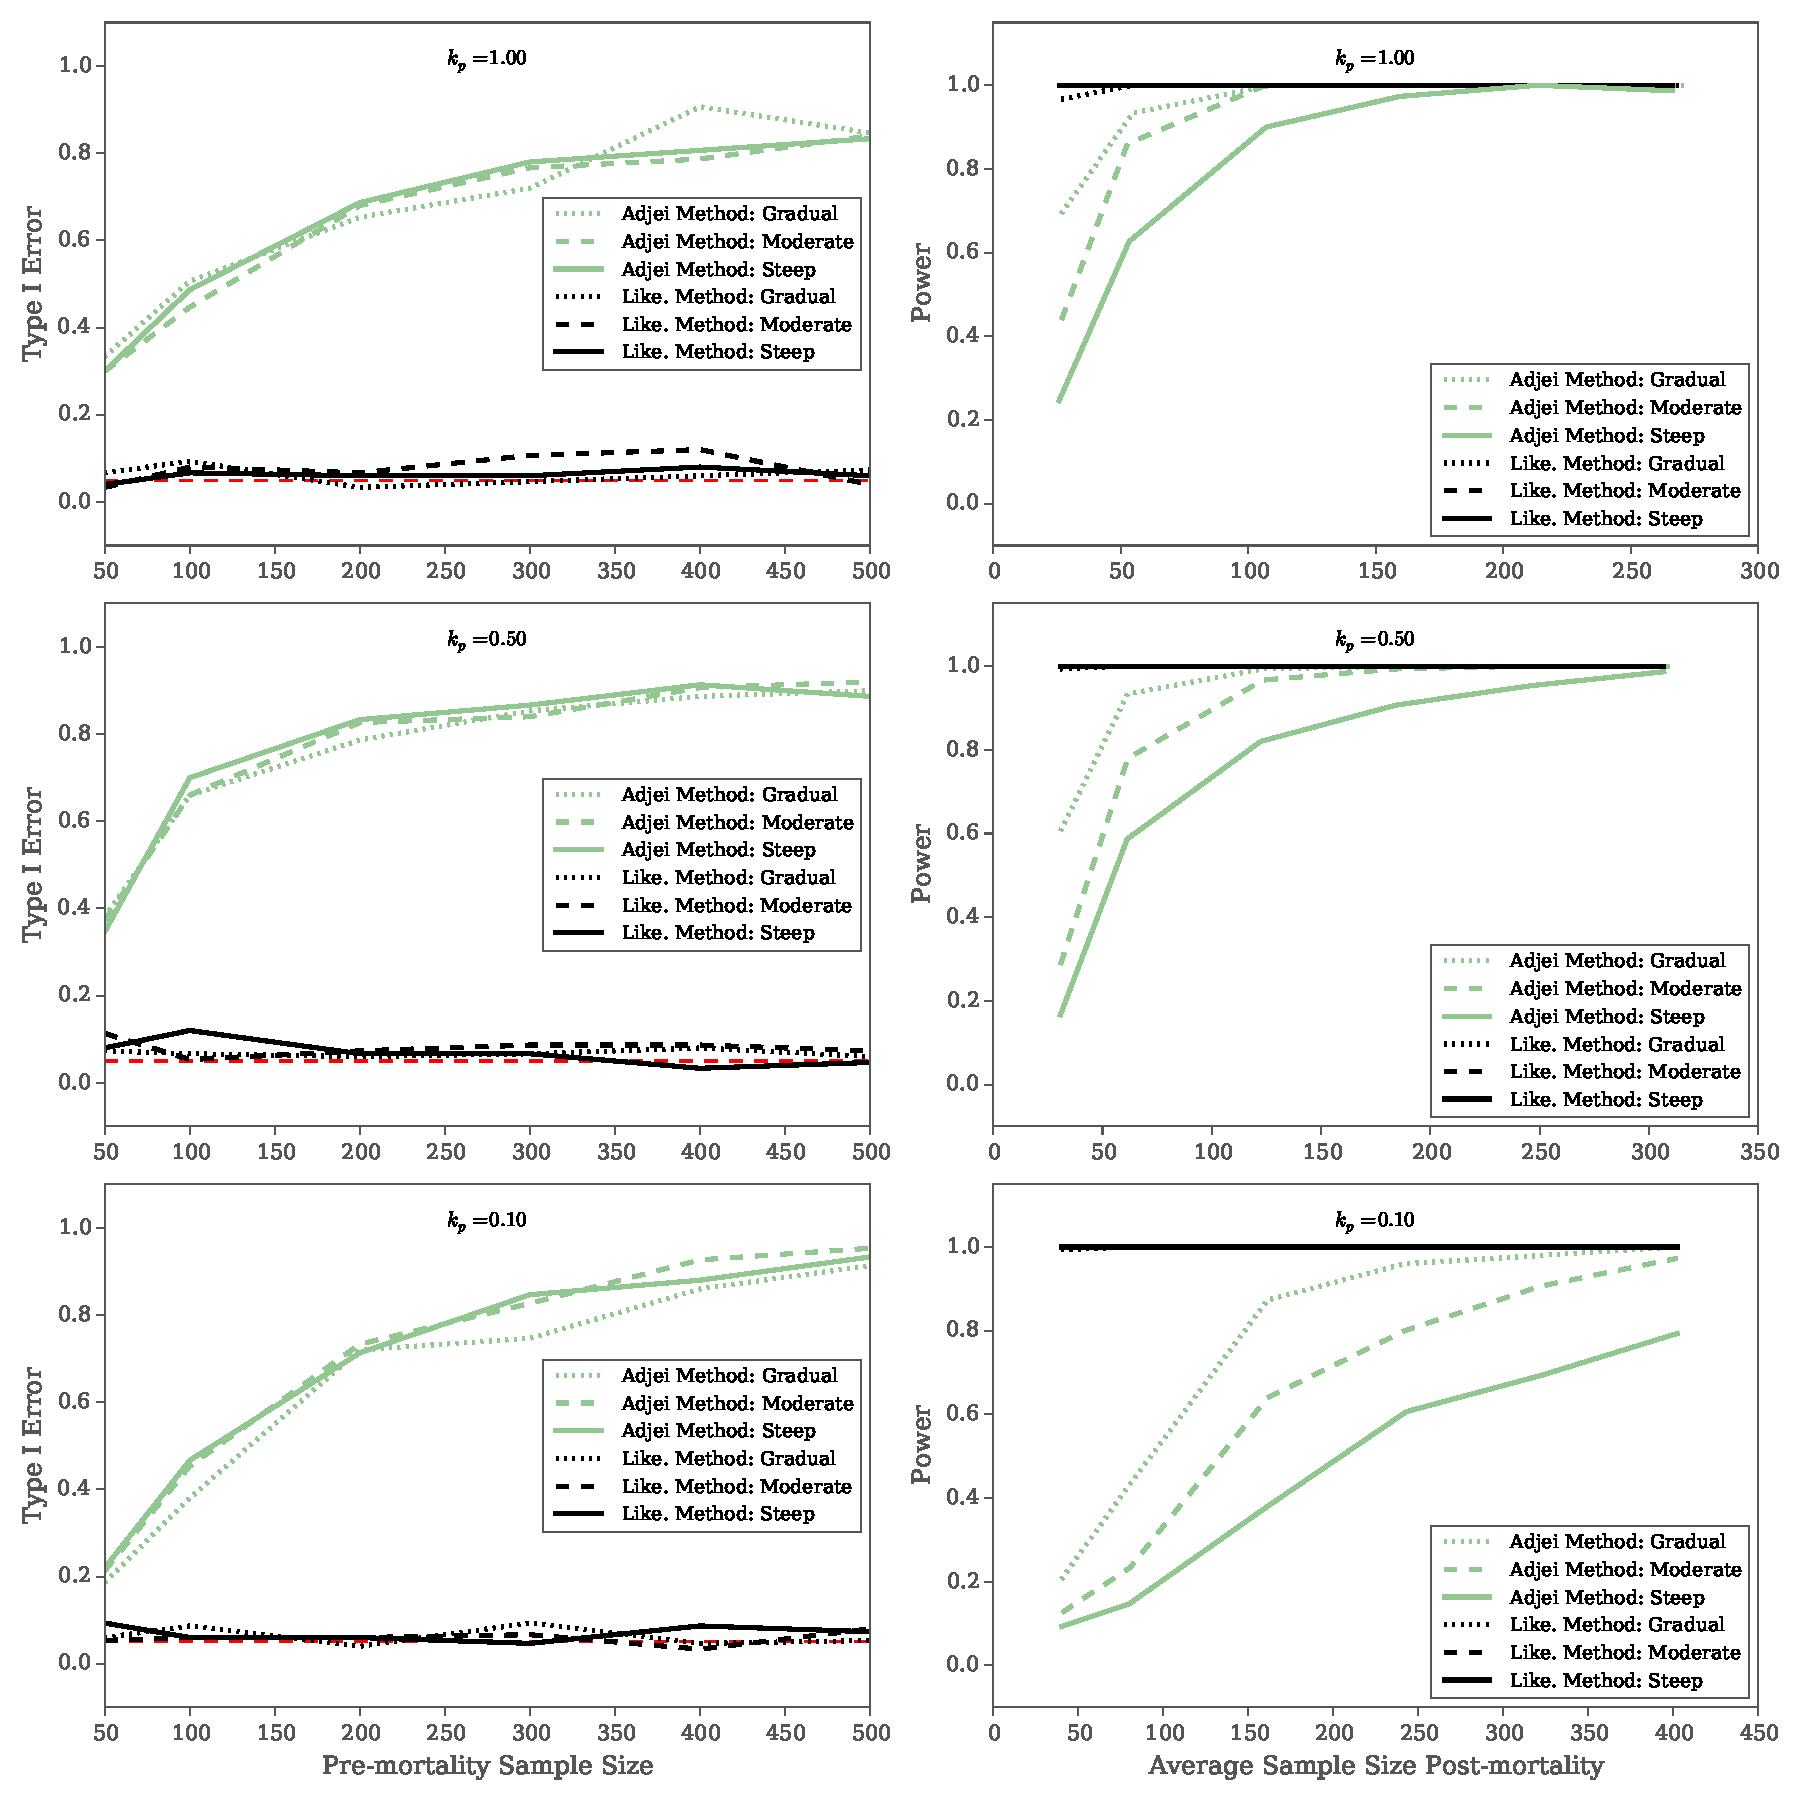
\includegraphics[width=\textwidth]{/Users/mqwilber/Repos/parasite_mortality/results/typeIpower_figure_for_mu10}

    \caption{The type I error rate and the power of the Likelihood Method (solid line) and the Adjei Method (dashed lines) when $\mu_p = 10$ for various shapes of the host survival function and levels of aggregation $k_p$.  The first column gives the type I error rate of each method for falsely detecting PIHM when none is present.  The red line gives the the pre-set type I error rate of $\alpha = 0.05$.  The second column gives the power of a given method to detect PIHM when it is actually occurring. }
    \label{fig:typeI10}

\end{figure}

\begin{figure}

    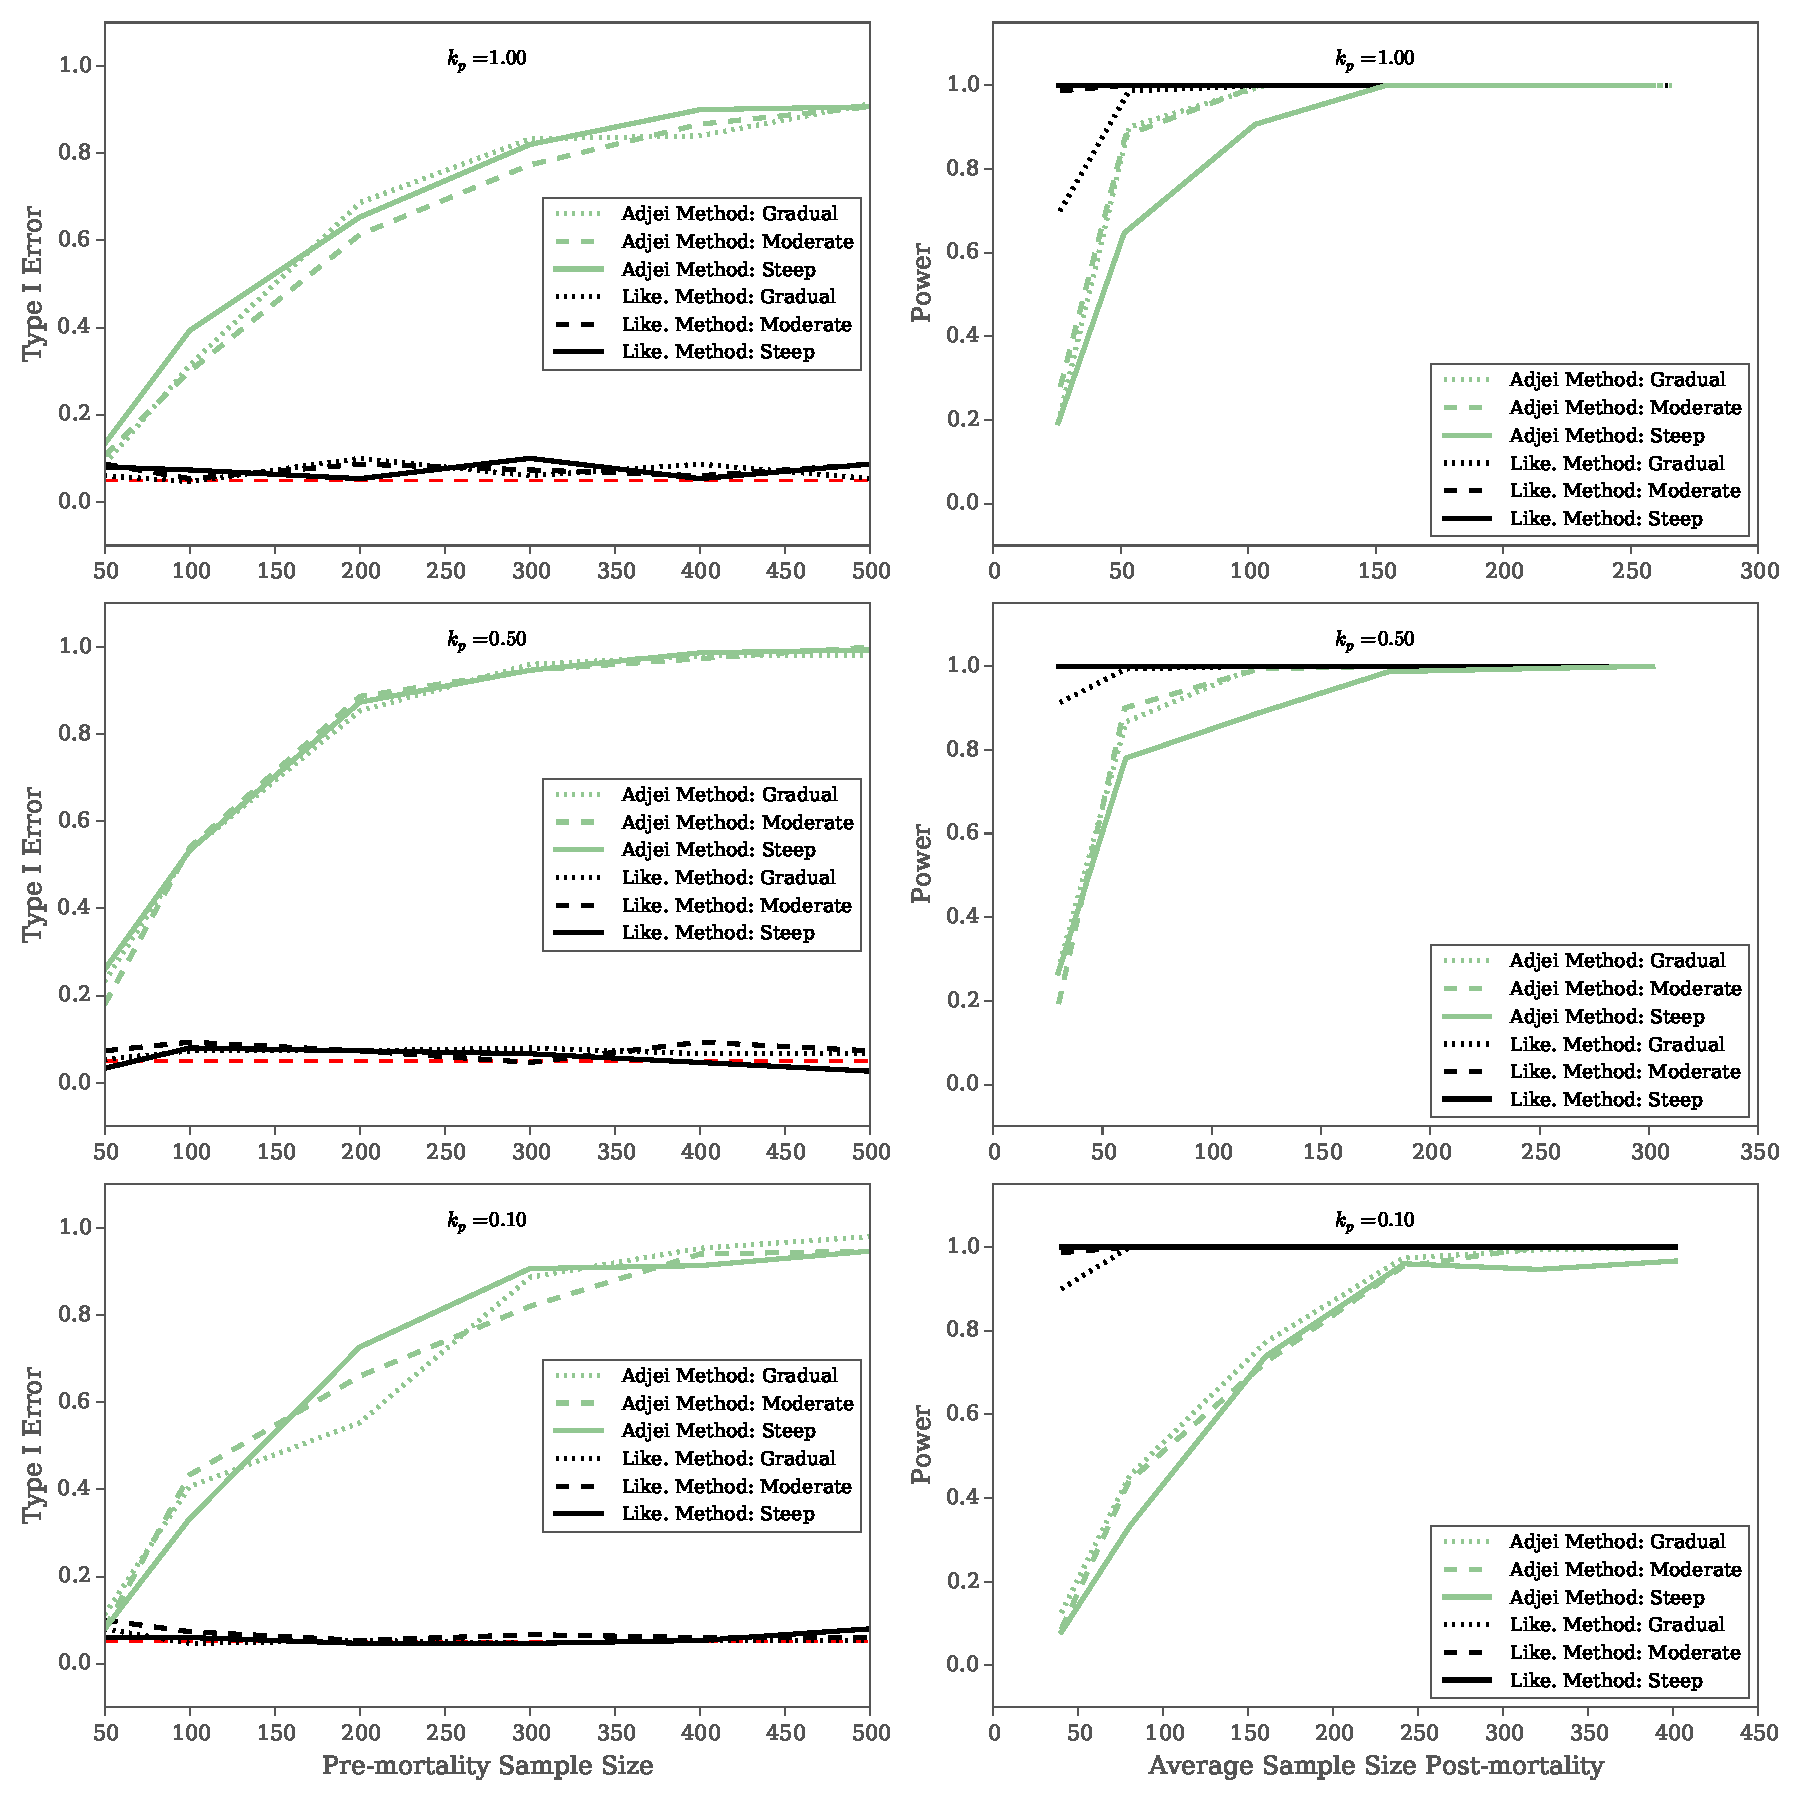
\includegraphics[width=\textwidth]{/Users/mqwilber/Repos/parasite_mortality/results/typeIpower_figure_for_mu50}

    \caption{The type I error rate and the power of the Likelihood Method (solid line) and the Adjei Method (dashed lines) when $\mu_p = 50$ for various shapes of the host survival function and levels of aggregation $k_p$.  The first column gives the type I error rate of each method for falsely detecting PIHM when none is present.  The red line gives the the pre-set type I error rate of $\alpha = 0.05$.  The second column gives the power of a given method to detect PIHM when it is actually occurring. }
    \label{fig:typeI50}

\end{figure}

\begin{figure}

    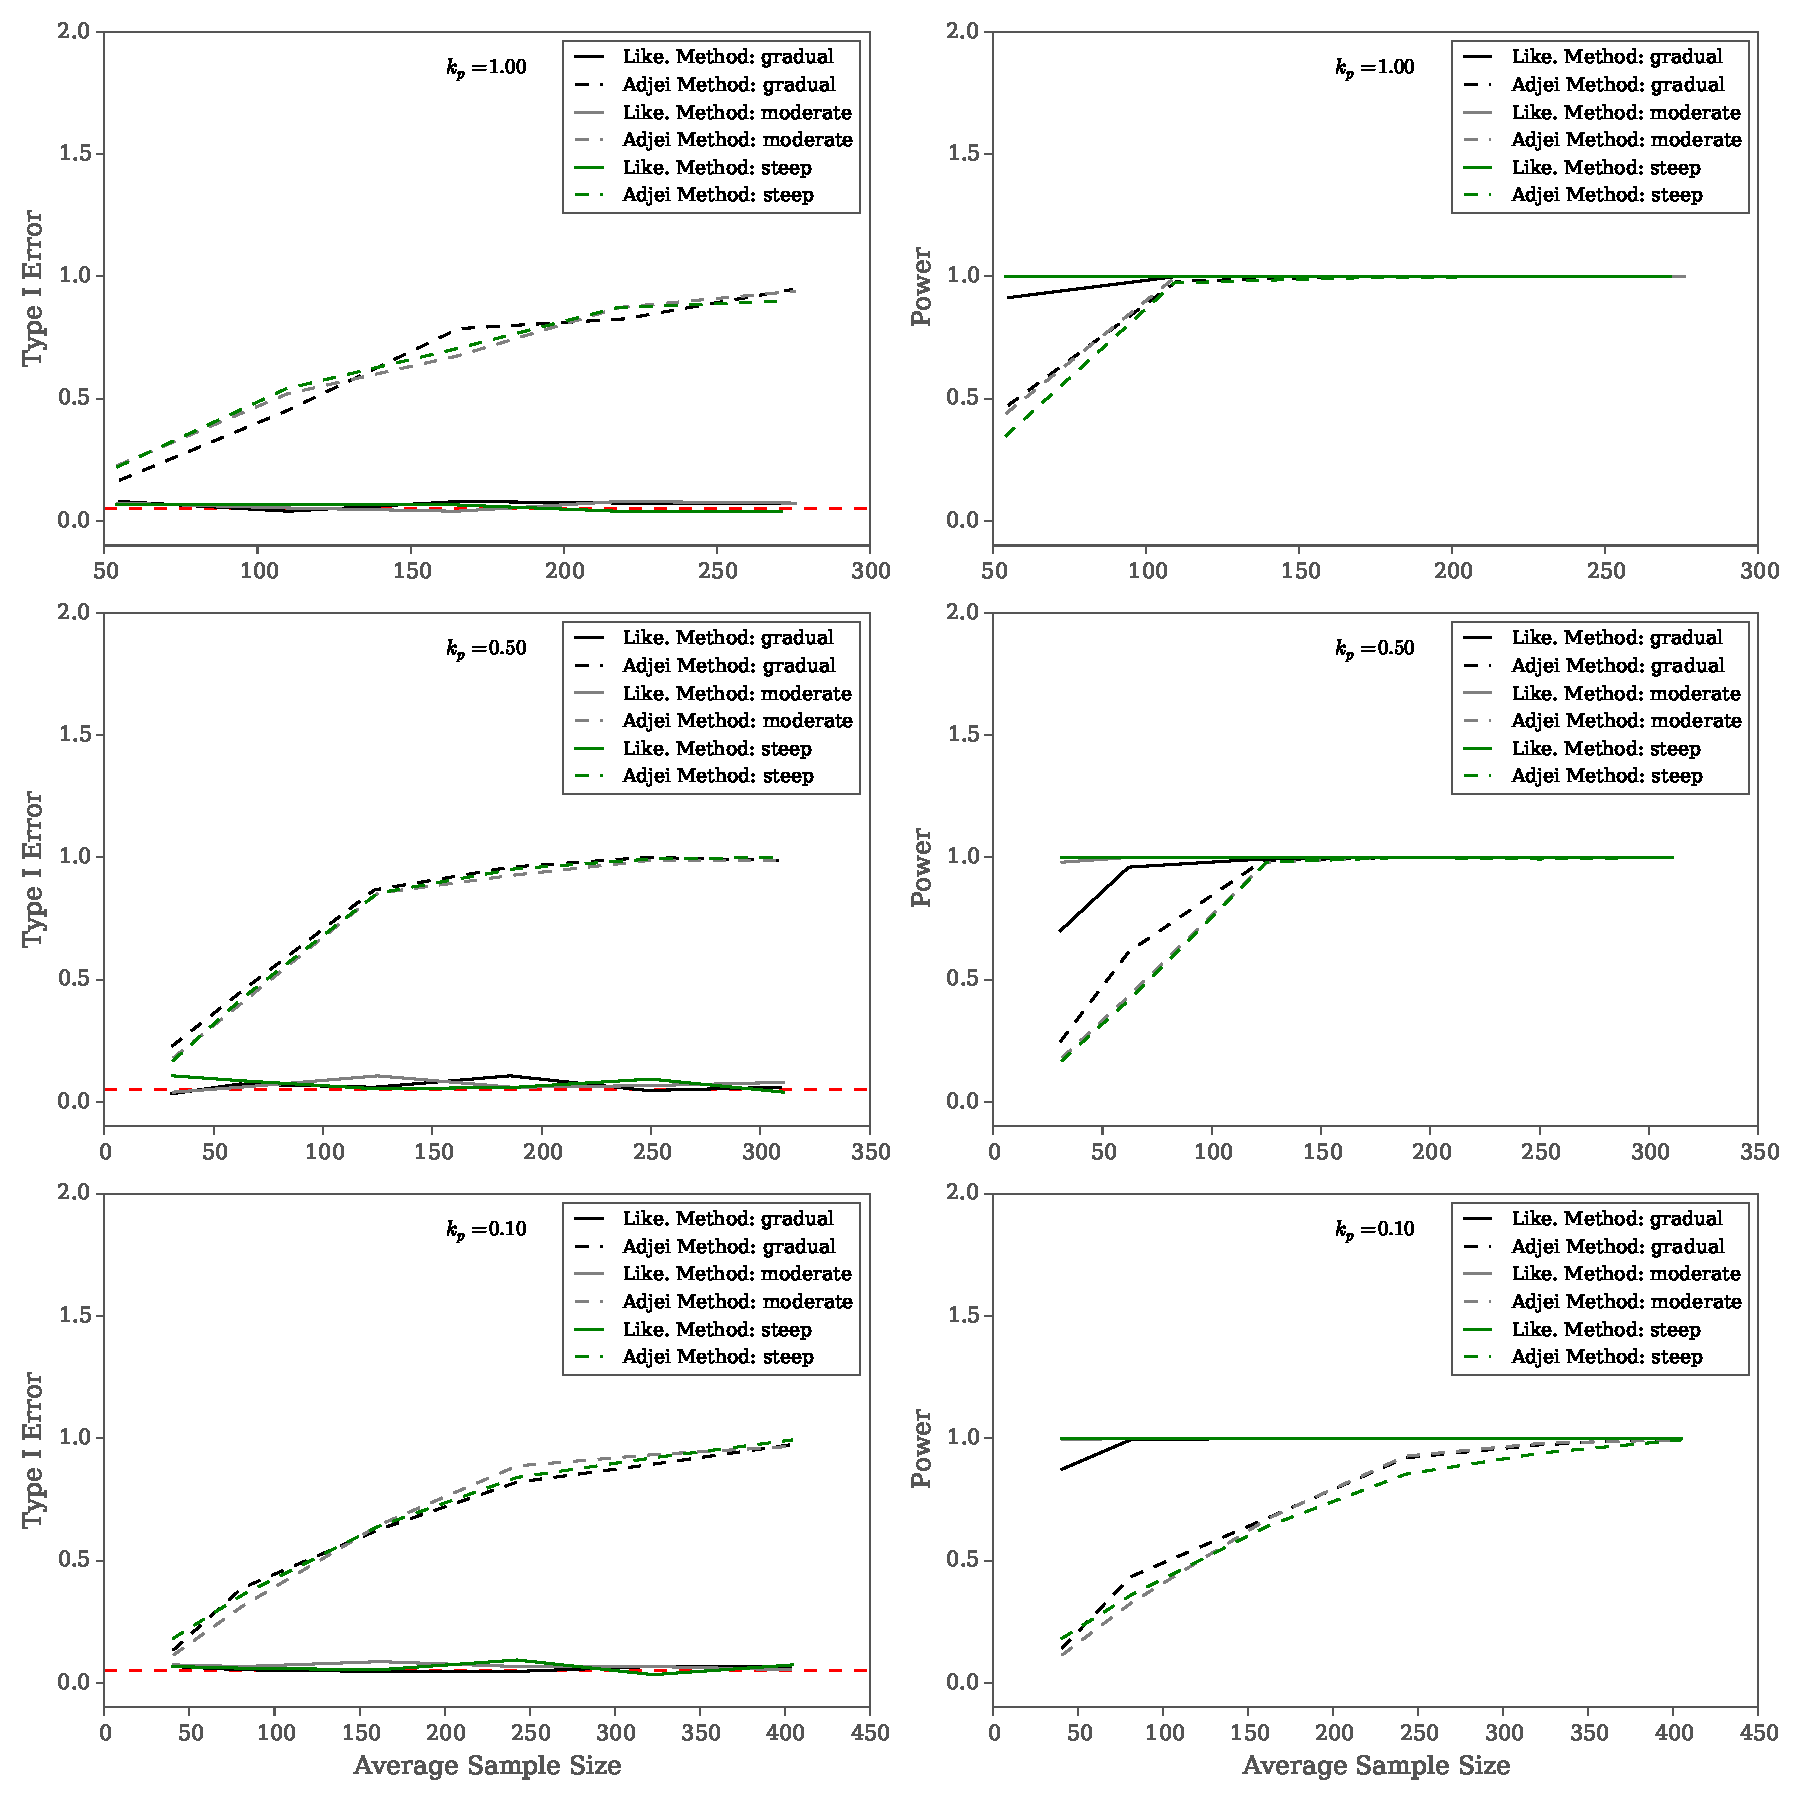
\includegraphics[width=\textwidth]{/Users/mqwilber/Repos/parasite_mortality/results/typeIpower_figure_for_mu100}

    \caption{The type I error rate and the power of the Likelihood Method (solid line) and the Adjei Method (dashed lines) when $\mu_p = 100$ for various shapes of the host survival function and levels of aggregation $k_p$.  The first column gives the type I error rate of each method for falsely detecting PIHM when none is present.  The red line gives the the pre-set type I error rate of $\alpha = 0.05$.  The second column gives the power of a given method to detect PIHM when it is actually occurring. }
    \label{fig:typeI100}

\end{figure}

\begin{figure}

    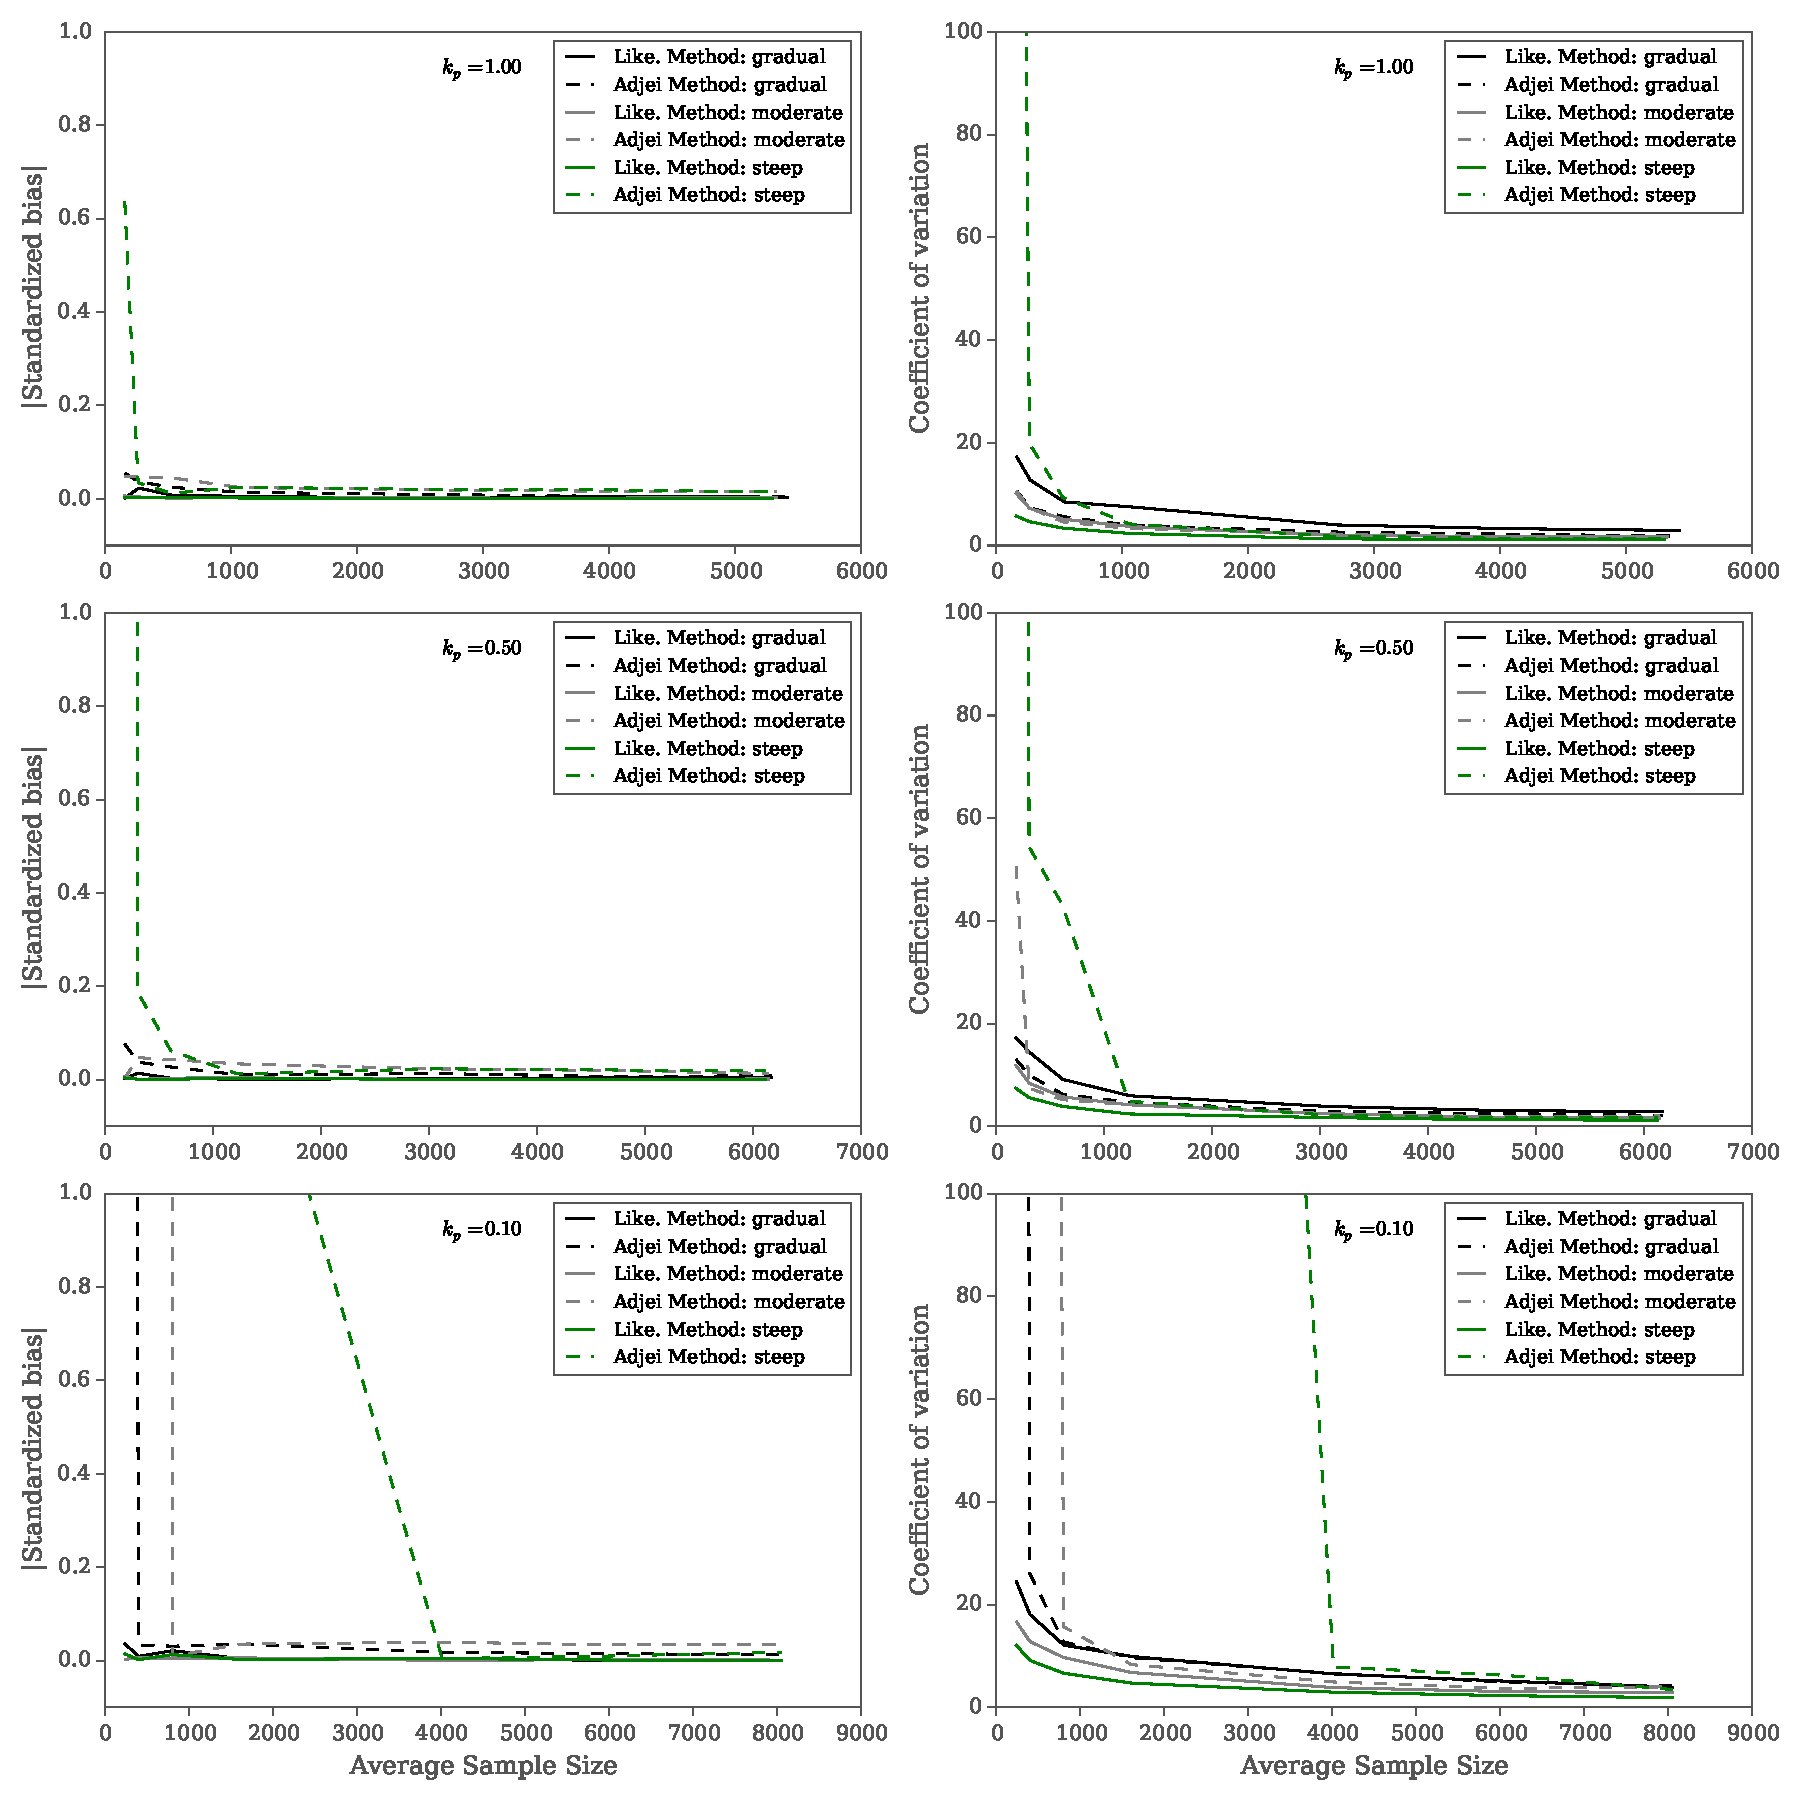
\includegraphics[width=\textwidth]{/Users/mqwilber/Repos/parasite_mortality/results/bais_prec_figure_for_ld50_mu10}

    \caption{The bias and the precision of the Likelihood Method (solid line) and the Adjei Method (dashed lines) when $\mu_p = 10$ for various shapes of the host survival function and levels of aggregation $k_p$ when estimating $LD_{50}$.  The first column gives the bias of each method's $LD_{50}$ estimate over 150 simulations. The second column gives the precision of each method's $LD_{50}$ estimate over 150 simulations.}

    \label{fig:biasld50_10}

\end{figure}

\begin{figure}

    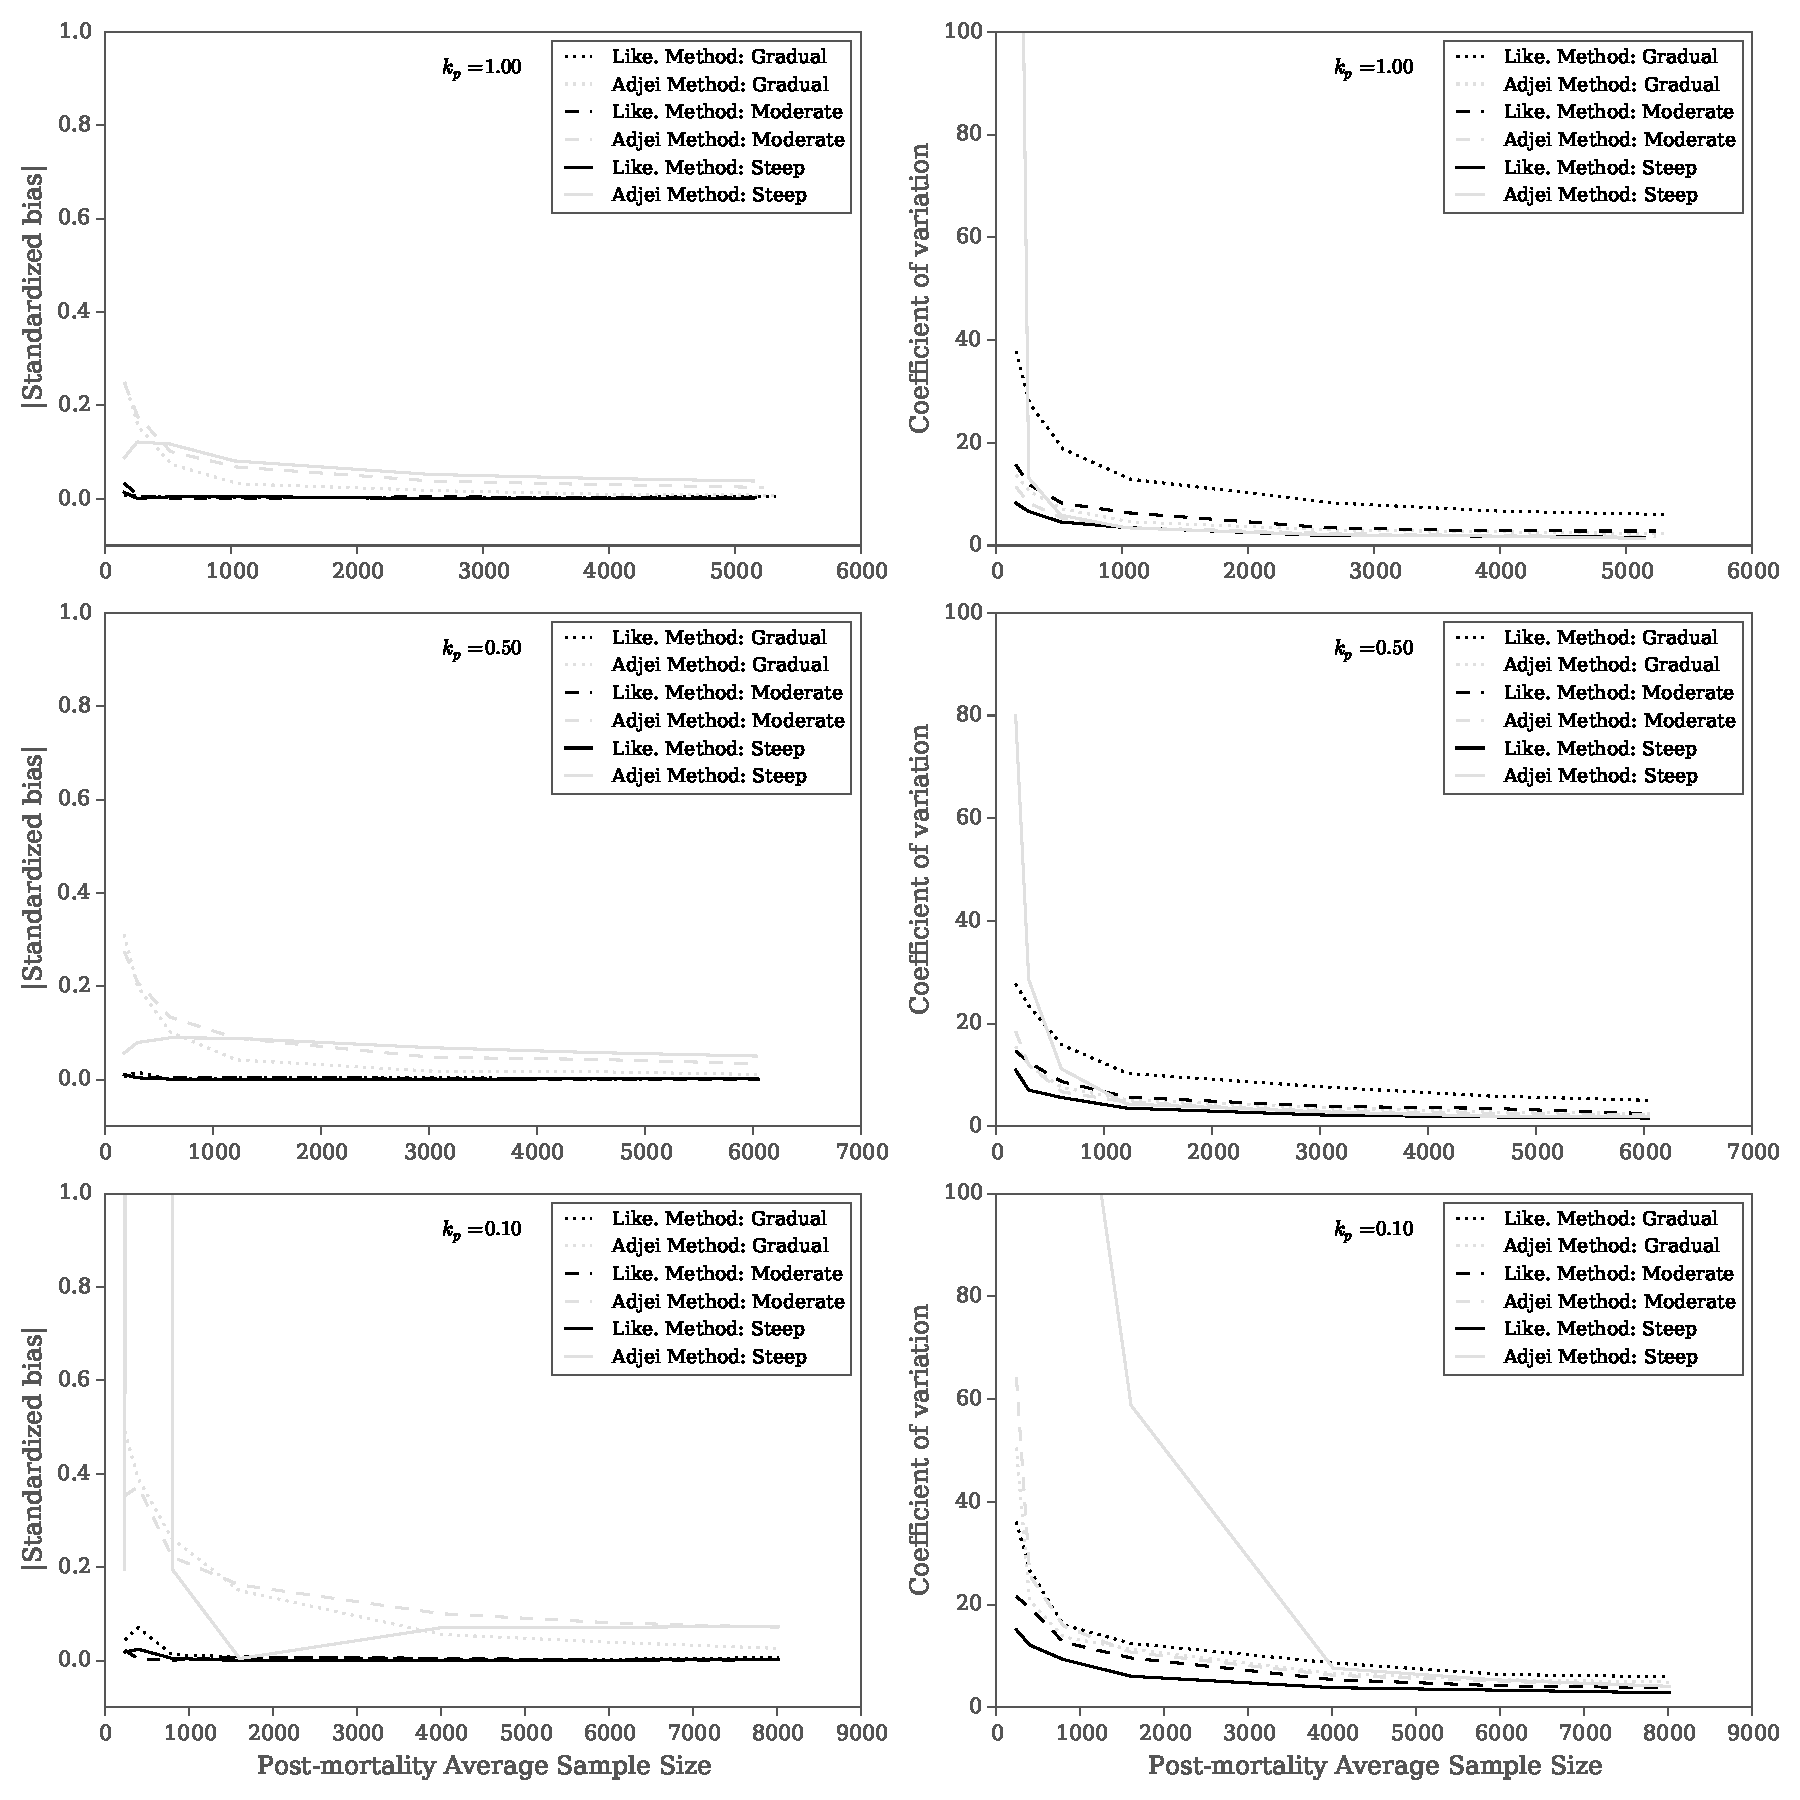
\includegraphics[width=\textwidth]{/Users/mqwilber/Repos/parasite_mortality/results/bais_prec_figure_for_ld50_mu50}

    \caption{The bias and the precision of the Likelihood Method (solid line) and the Adjei Method (dashed lines) when $\mu_p = 50$ for various shapes of the host survival function and levels of aggregation $k_p$ when estimating $LD_{50}$.  The first column gives the bias of each method's $LD_{50}$ estimate over 150 simulations. The second column gives the precision of each method's $LD_{50}$ estimate over 150 simulations.}

    \label{fig:biasld50_50}

\end{figure}

\begin{figure}

    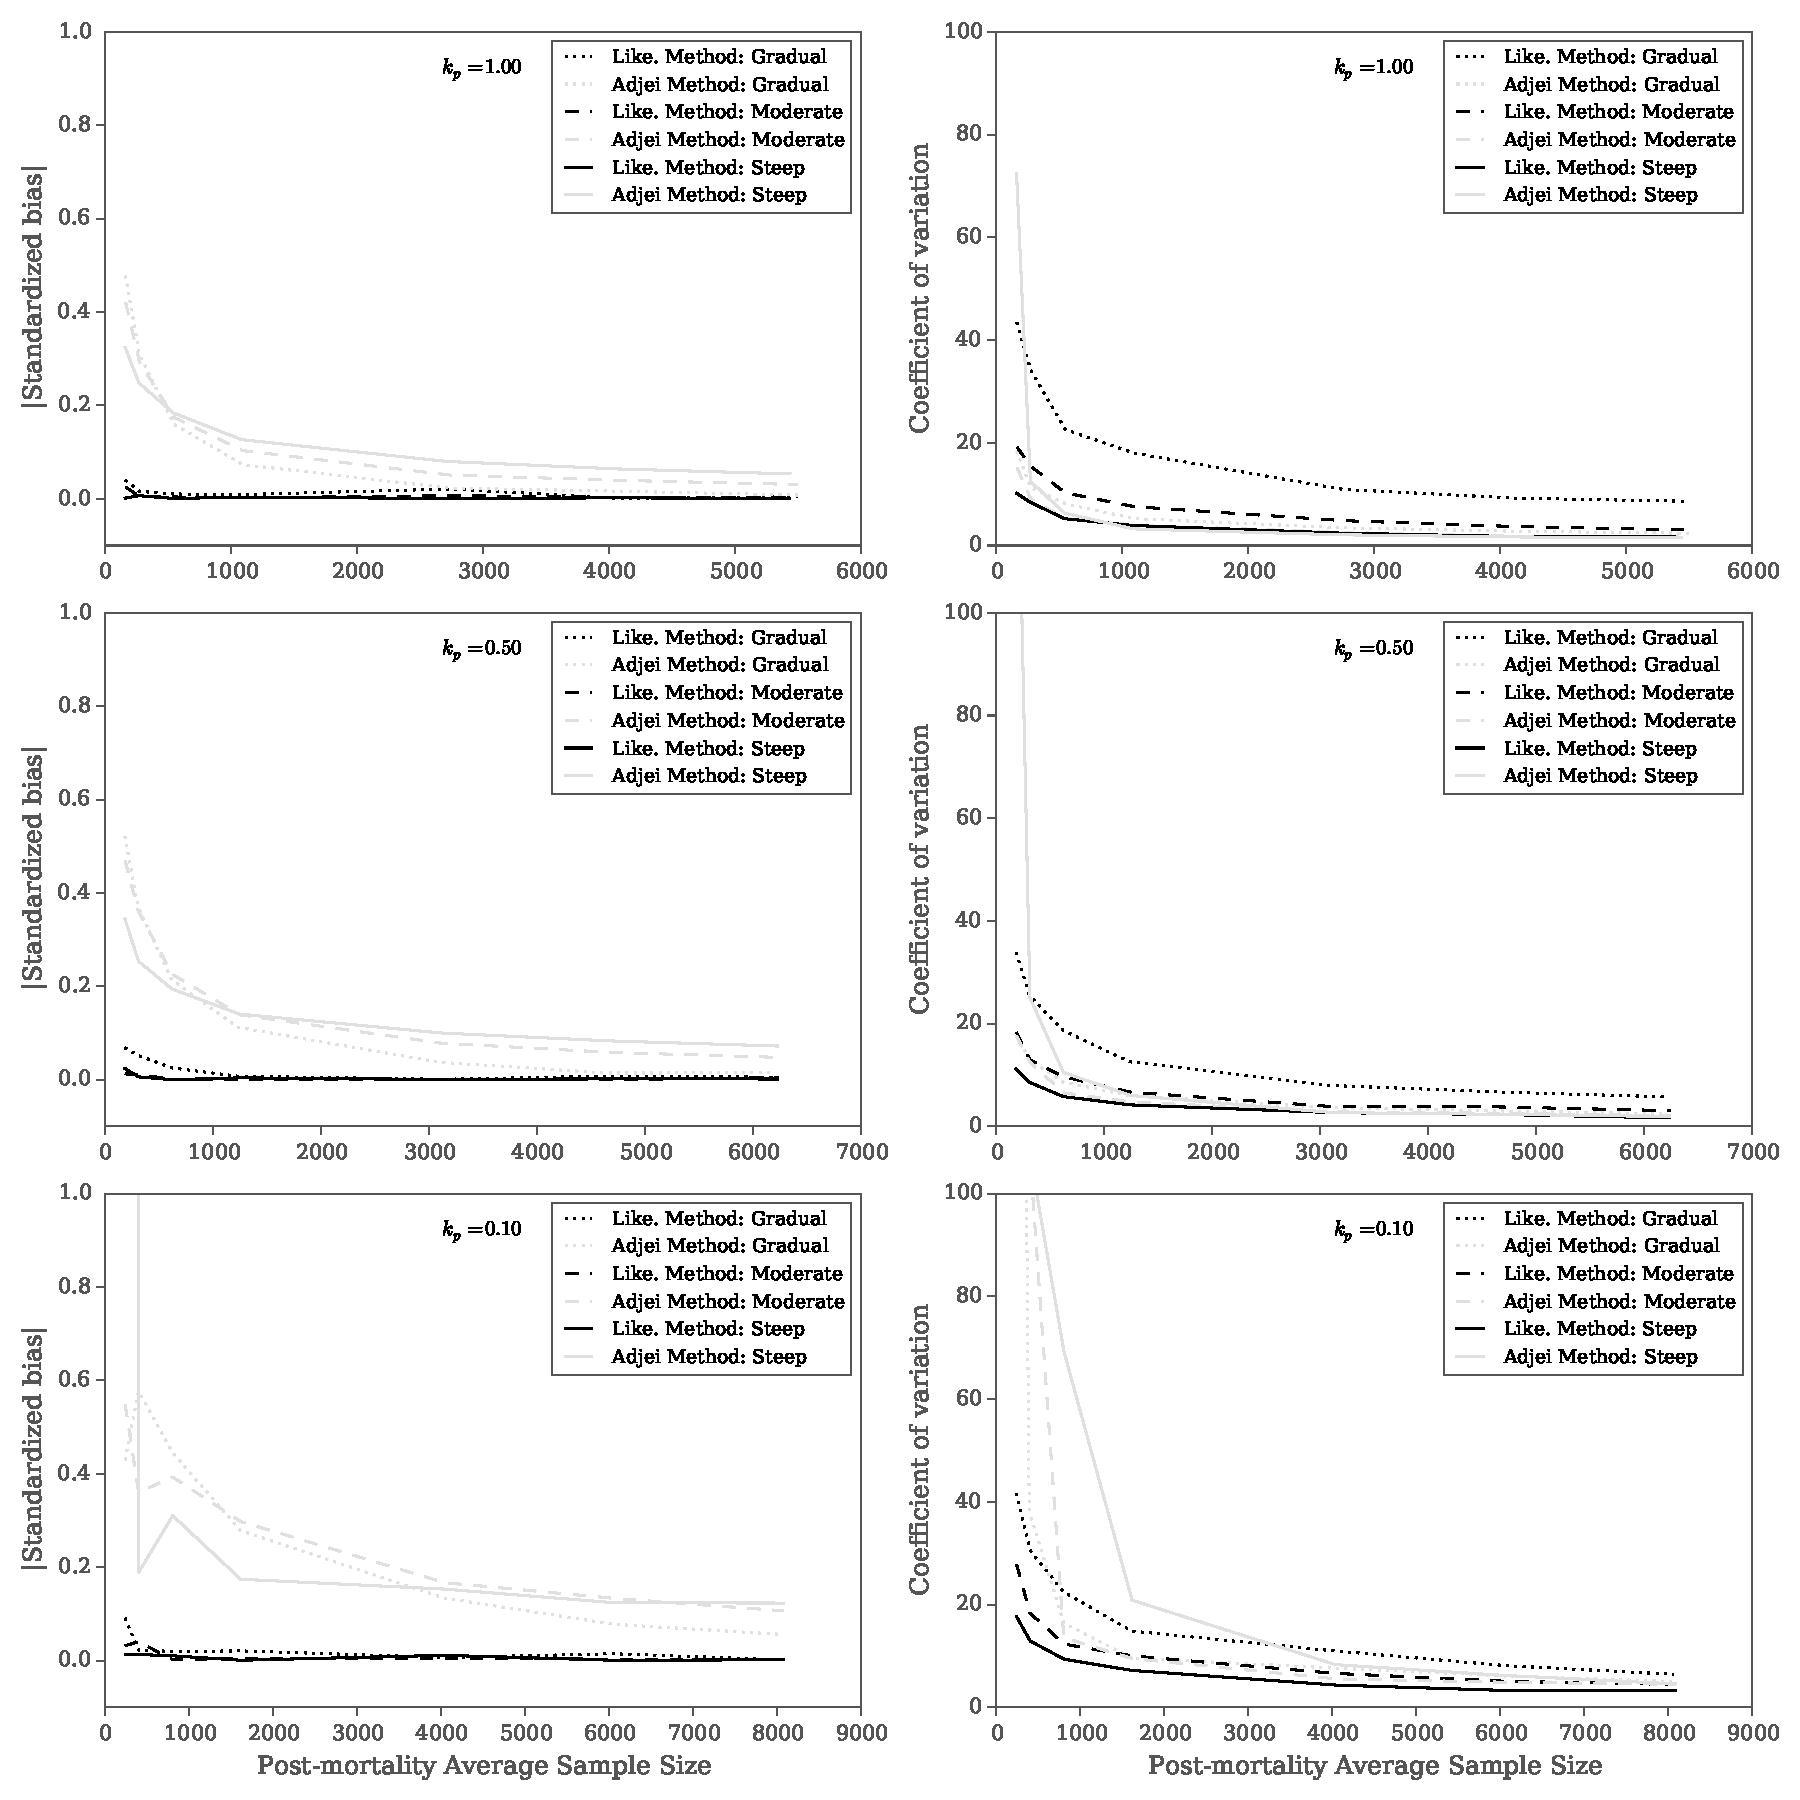
\includegraphics[width=\textwidth]{/Users/mqwilber/Repos/parasite_mortality/results/bais_prec_figure_for_ld50_mu100}

    \caption{The bias and the precision of the Likelihood Method (solid line) and the Adjei Method (dashed lines) when $\mu_p = 100$ for various shapes of the host survival function and levels of aggregation $k_p$ when estimating $LD_{50}$.  The first column gives the bias of each method's $LD_{50}$ estimate over 150 simulations. The second column gives the precision of each method's $LD_{50}$ estimate over 150 simulations.}

    \label{fig:biasld50_100}

\end{figure}

\begin{figure}

    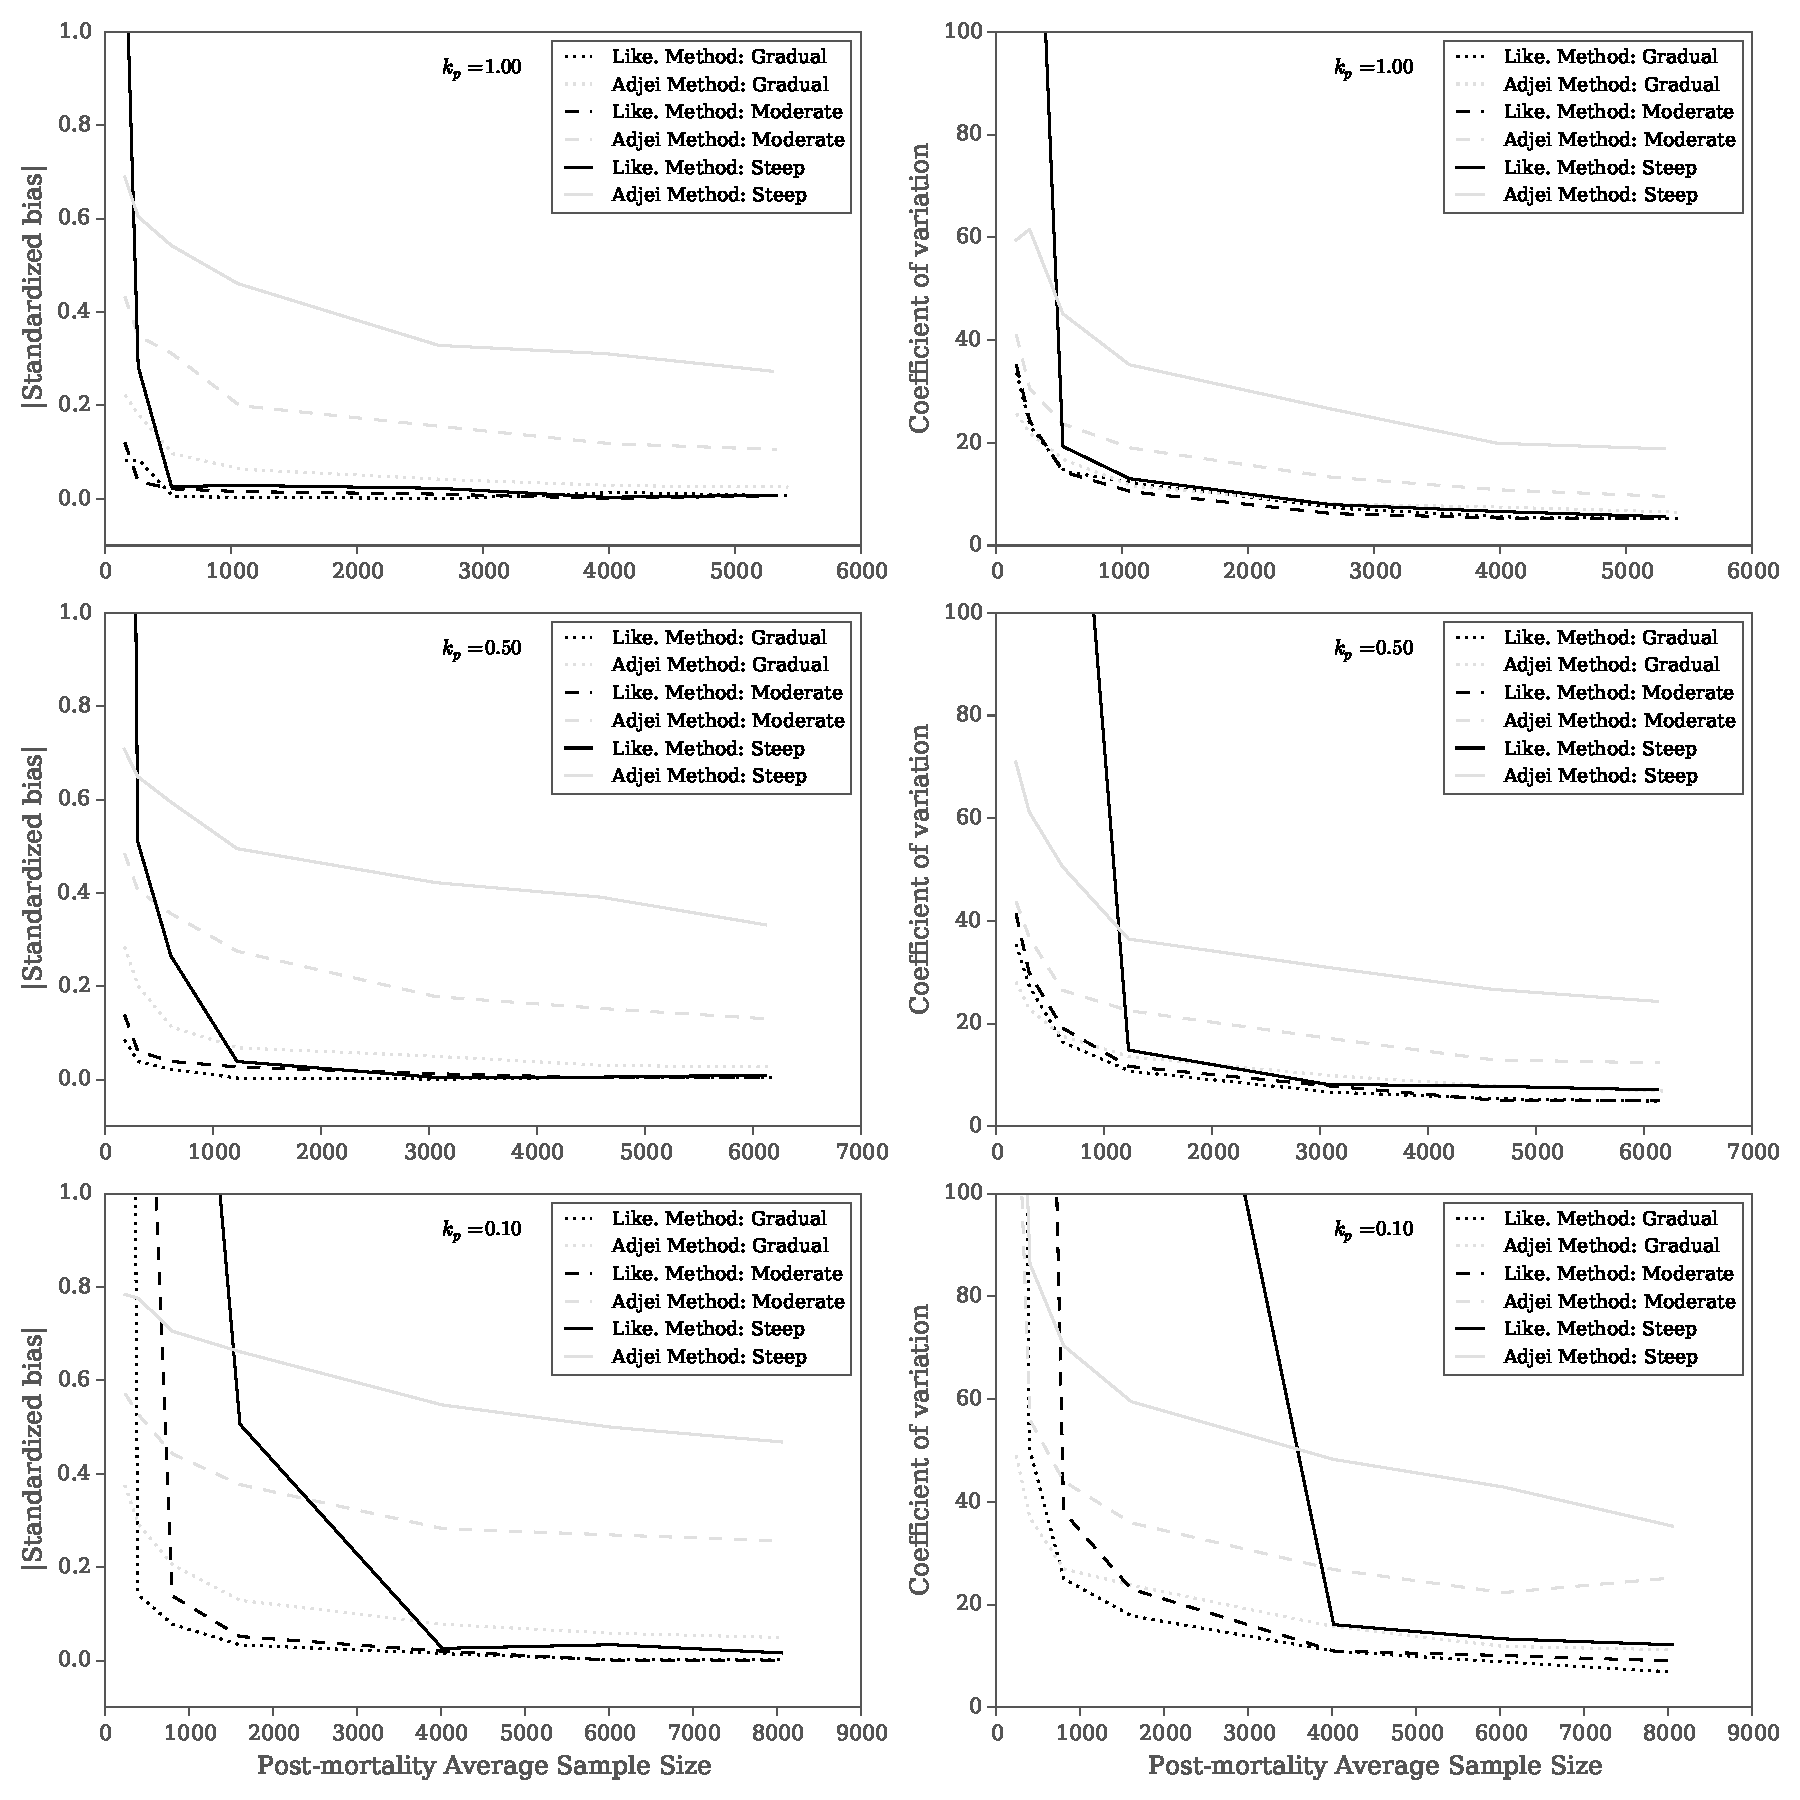
\includegraphics[width=\textwidth]{/Users/mqwilber/Repos/parasite_mortality/results/bais_prec_figure_for_a_mu10}

    \caption{The bias and the precision of the Likelihood Method (solid line) and the Adjei Method (dashed lines) when $\mu_p = 10$ for various shapes of the host survival function and levels of aggregation $k_p$ when estimating the $a$ parameter of the host survival function.  The first column gives the bias of each method's $a$ estimate over 150 simulations. The second column gives the precision of each method's $a$ estimate over 150 simulations.}

    \label{fig:biasa_10}

\end{figure}

\begin{figure}

    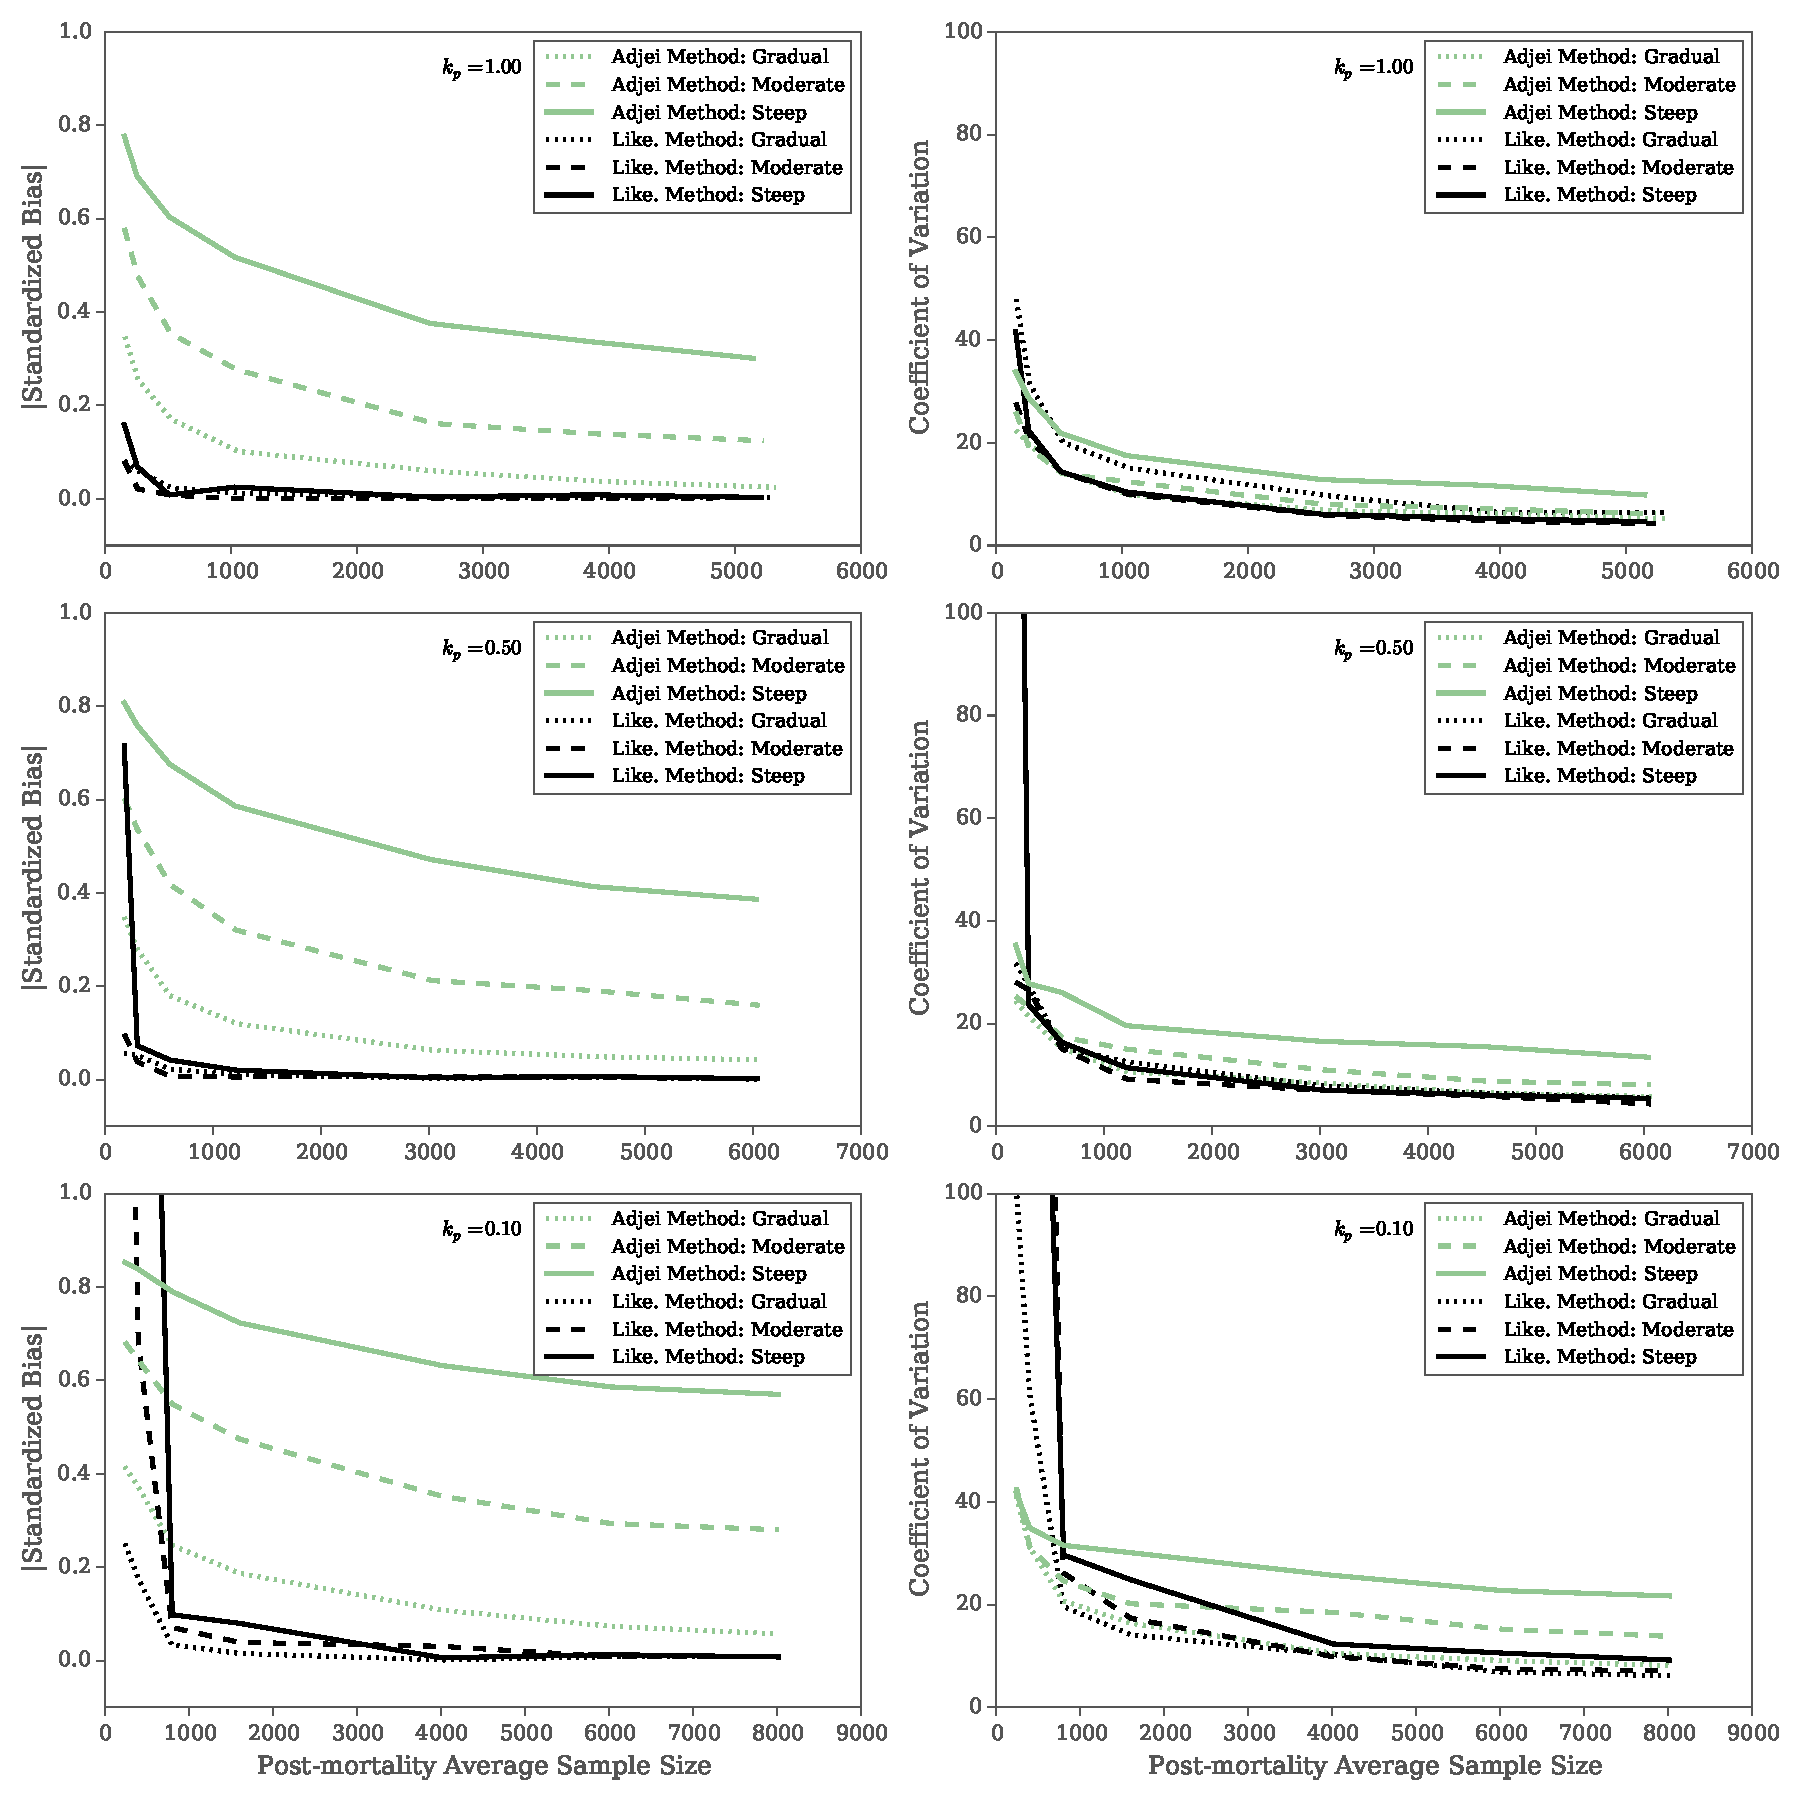
\includegraphics[width=\textwidth]{/Users/mqwilber/Repos/parasite_mortality/results/bais_prec_figure_for_a_mu50}

    \caption{The bias and the precision of the Likelihood Method (solid line) and the Adjei Method (dashed lines) when $\mu_p = 50$ for various shapes of the host survival function and levels of aggregation $k_p$ when estimating the $a$ parameter of the host survival function.  The first column gives the bias of each method's $a$ estimate over 150 simulations. The second column gives the precision of each method's $a$ estimate over 150 simulations.}

    \label{fig:biasa_50}

\end{figure}

\begin{figure}

    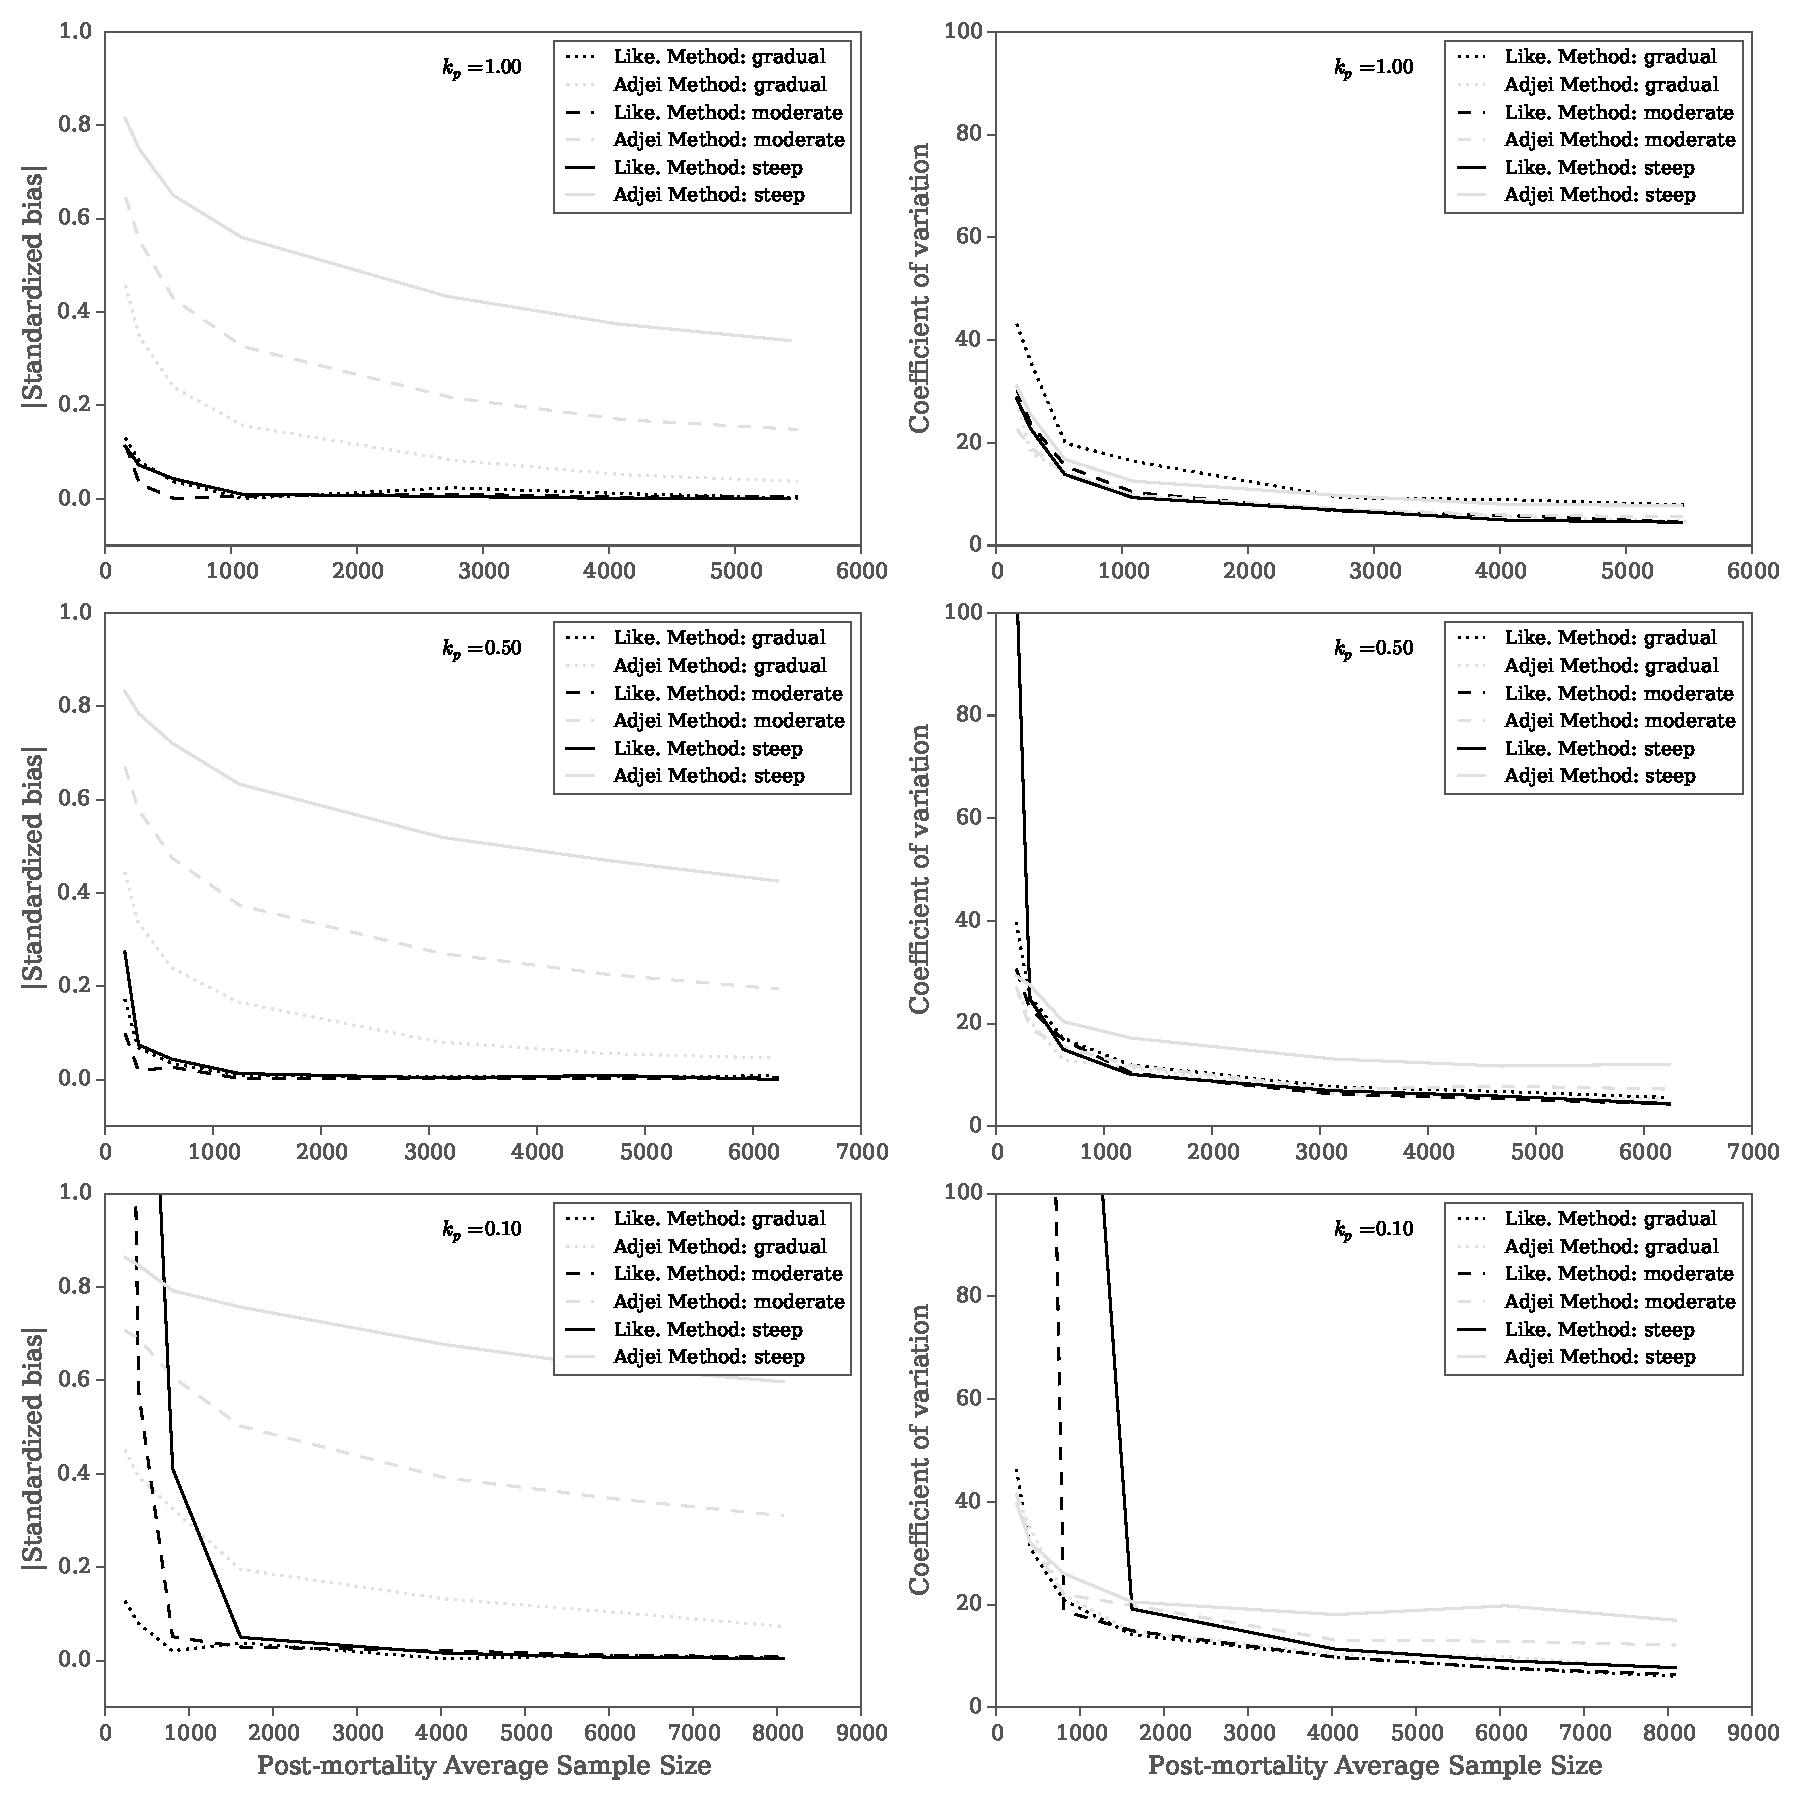
\includegraphics[width=\textwidth]{/Users/mqwilber/Repos/parasite_mortality/results/bais_prec_figure_for_a_mu100}

    \caption{The bias and the precision of the Likelihood Method (solid line) and the Adjei Method (dashed lines) when $\mu_p = 100$ for various shapes of the host survival function and levels of aggregation $k_p$ when estimating the $a$ parameter of the host survival function.  The first column gives the bias of each method's $a$ estimate over 150 simulations. The second column gives the precision of each method's $a$ estimate over 150 simulations.}

    \label{fig:biasa_100}

\end{figure}

\begin{figure}
    \centering
    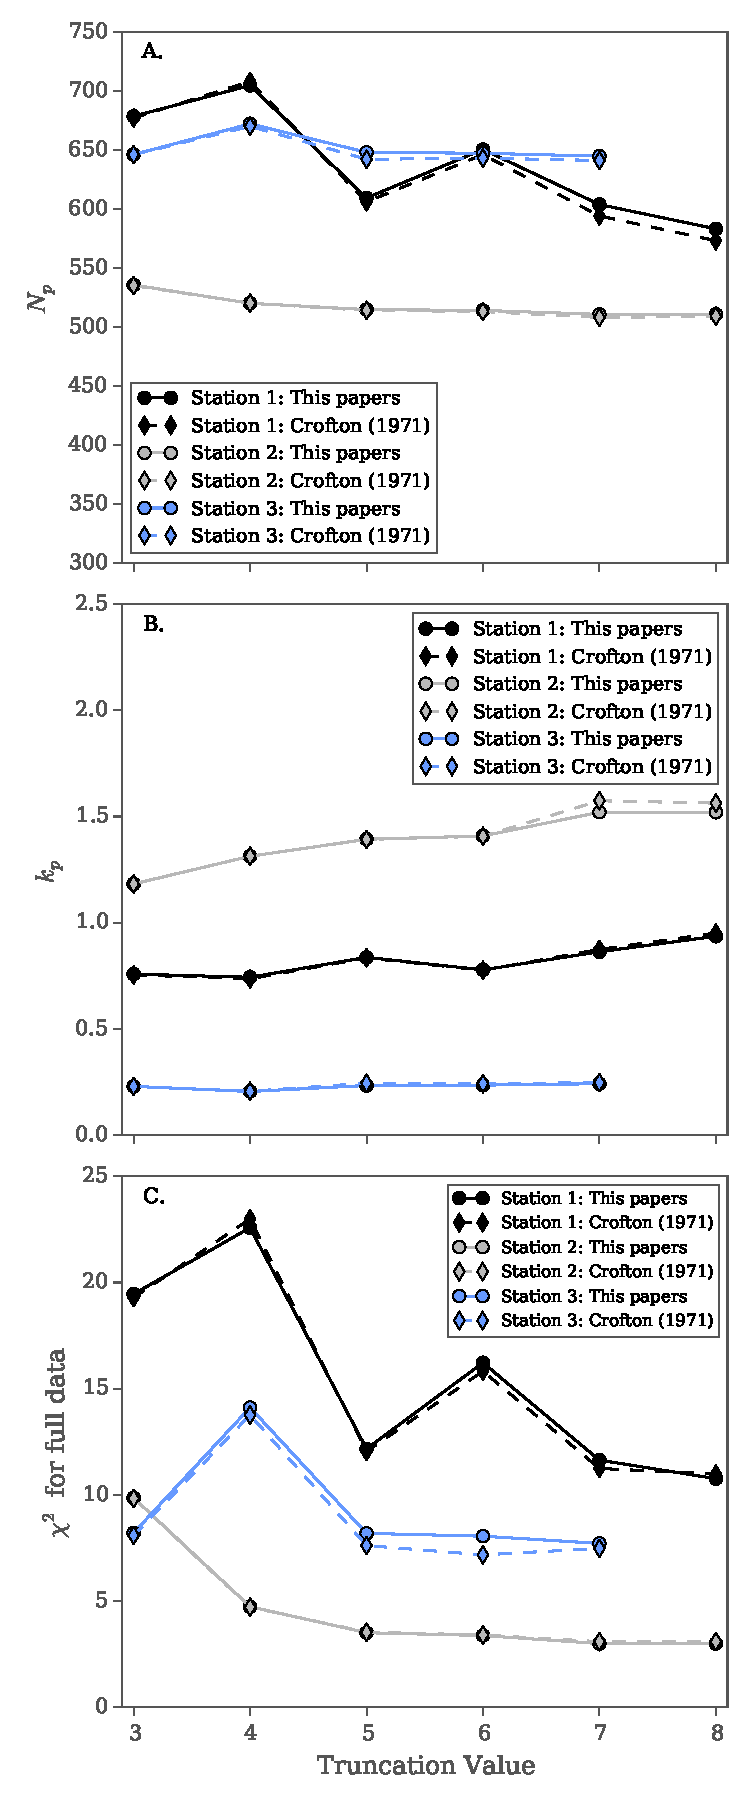
\includegraphics[width=0.5\textwidth]{/Users/mqwilber/Repos/parasite_mortality/results/compare_crofton.pdf}
    \caption{A comparison of this papers implementation (solid line, circles) of the Crofton Method with the results given in \cite{Crofton1971a} (dashed line, diamonds).  Figure A compares the predicted number of hosts in a population pre-mortality ($N_p$). Figure B compares the predicted parasite aggregation pre-mortality ($k_p$).  Figure C compares the $\chi^2$ statistic for each implementation.  Three of the 6 stations fit by \citeauthor{Crofton1971a} are shown here and all show that our implementation gives very similar results to those given by \citeauthor{Crofton1971a}.}
    \label{fig:crof_test}

\end{figure}



\singlespacing
\bibliographystyle{/Users/mqwilber/Dropbox/Documents/Bibformats/ecology_letters.bst}
\bibliography{/Users/mqwilber/Dropbox/Documents/Bibfiles/Projects_and_Permits-parasite_host_mortality}

\end{document}

